\documentclass[10pt]{article}

% 首先加载基础包
\usepackage[utf8]{inputenc}
\usepackage[T1]{fontenc}
\usepackage{multirow}
\usepackage{microtype}
\usepackage{graphicx}
\usepackage{amsfonts}
\usepackage{booktabs}
\usepackage{nicefrac}
\usepackage{doi}
\usepackage{float}
\usepackage{caption}
\usepackage[subrefformat=parens]{subcaption}
\usepackage{enumitem}
\usepackage{listings}

% tikz相关
\usepackage{tikz}
\usetikzlibrary{positioning,arrows.meta,shapes,backgrounds,fit}

% hyperref和url
\usepackage{url}
\usepackage{hyperref}

% arxiv包
\usepackage{arxiv}

% 其他可选包
\usepackage{lipsum}
\usepackage[
    backend=bibtex,
    style=numeric,
    sorting=none
]{biblatex}
\addbibresource{references.bib}

% Remove any spaces from the .bib file paths
\DeclareNameAlias{default}{family-given}

\title{Efficient Small Object Detection YOLO Model for Edge Computing}

%\date{September 9, 1985}	% Here you can change the date presented in the paper title
%\date{} 					% Or removing it

\author{
    \href{https://orcid.org/0009-0000-4164-8952}{\protect\noindent
\includegraphics[scale=0.06]{orcid.pdf}\hspace{1mm}Jinze Huang}\thanks{Supervise the research project, conceptualize the methodology, and lead the experimental design and implementation}\\
    Department of Computer Science\\
    New York University\\
    New York, USA\\
    \texttt{jh9108@nyu.edu}\\
    \And
    Ning Miao\thanks{Contribute to experimental design and implementation, improve the model architecture, and handle the documentation}\\
    Courant Institute of Mathematical Sciences\\
    New York University\\
    New York, USA\\
    \texttt{nm4543@nyu.edu}
}

% Uncomment to remove the date
\date{}

% Uncomment to override  the `A preprint' in the header
\renewcommand{\headeright}{Research Report}
%\renewcommand{\undertitle}{Technical Report}
% \renewcommand{\shorttitle}{\textit{arXiv} Template}

%%% Add PDF metadata to help others organize their library
%%% Once the PDF is generated, you can check the metadata with
%%% $ pdfinfo template.pdf
% \hypersetup{
% pdftitle={A template for the arxiv style},
% pdfsubject={q-bio.NC, q-bio.QM},
% pdfauthor={David S.~Hippocampus, Elias D.~Striatum},
% pdfkeywords={First keyword, Second keyword, More},
% }

\usepackage{amsmath}
\usepackage{amssymb}
\usepackage{bm}

\begin{document}
\maketitle

\begin{abstract}
    This research focuses on enhancing real-time small object detection (SOD) on edge devices by modifying the YOLOv8s architecture. We address the challenges of detecting small objects, particularly traffic signs in the TT100K dataset, by integrating a Global Attention Module (GAM) and optimizing the detection heads for shallow features (P2/3/4) and removing P5. Our proposed model achieves a mAP50 of 0.91226, a 58.8\% improvement over the baseline. Model compression techniques, including pruning and INT8 quantization, are also investigated, yielding up to a sixfold increase in inference speed on an NVIDIA A100 GPU with minimal accuracy loss, which reduce model from 10.0M to 5.46M, GFLOPS from 102.4 to 50.7, and inference speed up to 6 times faster with acceptable metrics loss. However, these reductions are less than 10\%. The proposed model outperforms other lightweight models and demonstrates significant potential for robust and efficient SOD in resource-constrained environments.
\end{abstract}


% keywords can be removed
\keywords{YOLO, Small Object Detection, Edge Computing, Attention Mechanism, Model Compression}


\section{Introduction}
With the rapid development of the computer vision field in recent years, object detection technology has become increasingly efficient and accurate. However, deploying efficient and accurate real-time small object detection algorithms in edge devices remains a challenge task. Concretely, small objects contain very few pixels, making feature extraction difficult. Also, many object detection algorithms need to resize the original input to a lower resolution form (e.g $640 \times 640$ pixels), When resizing high resolution images, small objects may lose critical information. Moreover, there is a technical contradiction, small objects detection need deeper networks but edge devices require lightweight models, so we need to do a trade-off.
Before neural networks were widely used, the mainstream of SOD algorithms was based on traditional image processing. It was highly relied on manual feature extraction\cite{xiuling2024} such as Haar features, HOG \cite{dollar2009pedestrian}, and etc. In the post-Neural Nerwork era, object detection algorithms based on CNN (convolution neural network) dominated the development of the object detection field. With diverse datasets and additional semantic information, the performance of SOD has been improved.

For SOD, an individual object usually only occupies a tiny part of the picture with low resolution, occlusion, and background noise. These characteristics make normal object detection models hard to identify tiny individuals, therefore, we need specific SOD technology to detect and localize tiny objects accurately. SOD focuses on addressing the object with low resolution and weak feature representation which is easily influenced by background noise. In contrast, normal object detection models are applied when an object occupies a relatively big part of the picture. Hence, SOD faces problems arising from higher rates of missed and false detection, and it needs more sophisticated feature extraction and multi-scale adaptation techniques to detect accurately\cite{li2024ltea,han2024small}. 

YOLO is a fast and efficient object detection algorithm widely used for real-time detection. By modifying its feature extraction and pyramid network modules, we can improve accuracy while keeping it lightweight enough for edge devices\cite{ni2024yolo}. The model's innovative backbone structure enables high-accuracy real-time detection even with limited computing resources. Recent improvements like YOLO-RET have shown promising results in edge computing scenarios by enhancing system responsiveness through localized processing\cite{ret2022}. With my research deadline approaching rapidly, I chose YOLO as it provides a good balance between performance and development time, while still allowing room for novel improvements in small object detection through careful architectural modifications.

In this research, we focus on the following works:

 \begin{enumerate}
    \item Modify the YOLO architecture by adjusting transformer-based and CNN-based backbone modules, neck and detection heads and feature map fusion to create a light-weight model balancing performance and speed.
    \item Attention module is compared and used to improve the detection accuracy.
    \item Train the modified YOLO model on the TT100K dataset\cite{zzl}, which contains small traffic signs in diverse conditions.
    \item Compare different modified YOLOv8 model's performance and conduct ablation experiments to validate the proposed changes.
    \item Lightweight model by quantization and pruning and test on V100, A100 and Orin AGX X.
\end{enumerate}


\section{Related Work}

\subsection{Small Object Detection}
In image processing, "small objects" are typically defined by their pixel area or relative size compared to the entire image. In this research, we define small objects as those with a pixel area less than $32 \times 32$ pixels or occupying less than 0.1\% of the total image area\cite{lin2014microsoft}. When the input image resolution is high, we need to downsample the high-resolution image to the network input size (e.g., $640 \times 640$ pixels) with a downsampling factor $s$. For an input image with dimensions $\bm{x} = (x_1, x_2)$, $\bm{x} \in \mathbb{R}^{H \times W}$, it becomes $\acute{\bm{x}} = (\acute{x_1}, \acute{x_2})$, $\acute{\bm{x}} \in \mathbb{R}^{\frac{H}{s} \times \frac{W}{s}}$. During this process, small objects may lose significant high-frequency information, making their features less distinct and harder to detect. The loss of high-frequency information during downsampling can be understood through Fourier transform. Images can be represented as a superposition of sine and cosine waves of different frequencies. High-frequency components correspond to fine details and small objects in the image. Downsampling causes these high-frequency components to be discarded or aliased, resulting in information loss.

\begin{equation}
  \acute{\bm{x}} = \text{Downsample}(\bm{x}, s)
  \label{eq:downsample}
\end{equation}

Due to the value of industry and society safety, small object detection(SOD) is always a hot spot in the object detection area.  Boshra Khalili and Andrew W.Smyth proposed an improved YOLOv8 by improving GFPN structure, adding c2-EMA modules, and modifying PIoU loss, achieving significant improvements in mAP0.5 from 40.6\% to 45.1\% in traffic CCTV.\cite{khalili2024sodyolo} Shi et al. proposed FocusDet in 2024, a specialized small object detection framework, integrating STCF-EANet backbone and Bottom FocusPAN, which improved mAP@.5 by 13.1\% and 6.2\% on VisDrone2021-DET and CCTSDB2021 datasets, respectively.\cite{shi2024focusdet} Remote sensing images also present significant challenges in object detection due to the prevalence of small-scale targets. Wang et al. introduced a novel arbitrary-oriented object detection framework for remote sensing images, incorporating a periodic pseudo-domain angle representation and ratio-balanced loss, achieving competitive results on multiple datasets.\cite{wang2023oriented} Comparasion of different object detection algorithms is shown in Fig. \ref{fig:object_detection_comparison}.

\subsection{Backbone}
Backbone in deep learning serves as the primary feature extractor network, responsible for processing input data and computing a hierarchical representation of features, which can then be utilized by subsequent task-specific modules for various applications such as object detection, segmentation, or classification.
Apple published a new Backbone called MobileOne\cite{lee2023efficient} in 2023. It reduced memory access cost(MAC) by forcing synchronization like global pooling used in Squeeze-Excite block, using skip connections and squeeze-excite blocks and different structure of training and inference. GhostNetV2 captured the dependence between long-range pixels by fully-connected(FC) layers to aggregate local and long-range information simultaneously.
\begin{figure}[H]
    \centering
    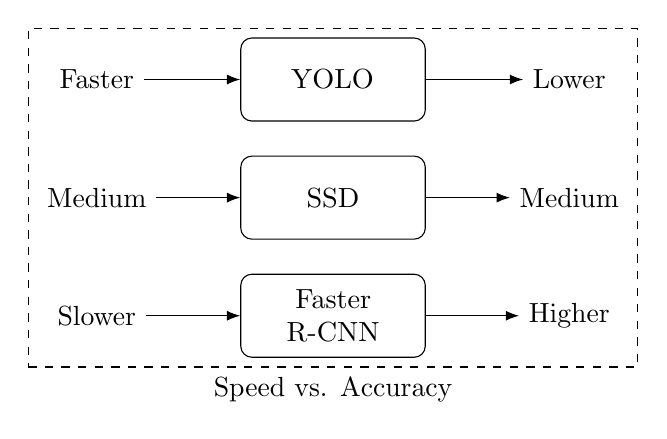
\begin{tikzpicture}[
        node distance = 1.5cm,
        block/.style = {rectangle, draw, text width=6em, text centered, rounded corners, minimum height=3em},
        line/.style = {draw, -{Latex}}
    ]
    
    \node [block] (yolo) {YOLO};
    \node [block, below of=yolo] (ssd) {SSD};
    \node [block, below of=ssd] (faster) {Faster R-CNN};
    
    \node [left of=yolo, node distance=3cm] (yolo_speed) {Faster};
    \node [right of=yolo, node distance=3cm] (yolo_acc) {Lower};
    \node [left of=ssd, node distance=3cm] (ssd_speed) {Medium};
    \node [right of=ssd, node distance=3cm] (ssd_acc) {Medium};
    \node [left of=faster, node distance=3cm] (faster_speed) {Slower};
    \node [right of=faster, node distance=3cm] (faster_acc) {Higher};

    \path [line] (yolo_speed) -- (yolo);
    \path [line] (yolo) -- (yolo_acc);
    \path [line] (ssd_speed) -- (ssd);
    \path [line] (ssd) -- (ssd_acc);
    \path [line] (faster_speed) -- (faster);
    \path [line] (faster) -- (faster_acc);

    \node[draw, dashed, fit=(yolo)(ssd)(faster)(yolo_speed)(yolo_acc)(ssd_speed)(ssd_acc)(faster_speed)(faster_acc), label=below:Speed vs. Accuracy] {};

    \end{tikzpicture}
    \caption{Comparison of Object Detection Algorithms (Speed vs. Accuracy)}
    \label{fig:object_detection_comparison}
\end{figure}

\subsection{Edge Computing}
With the proliferation of the Internet of Things (IoT), edge computing has emerged to meet the demand for faster and more reliable data processing. The core principle of edge computing is to deploy computational resources closer to devices, reducing transmission latency and enhancing data processing efficiency.
Qiu et al.\cite{electronics13163269} proposed LD-YOLOv10, a lightweight drone target detection algorithm that incorporates a novel RGELAN feature extraction structure, an AIFI module with multi-head attention, a DR-PAN Neck structure, and a combination of Wise-IoU and EIoU loss functions.
Liu et al.\cite{liu2023edgeyolo} proposed a lighter decoupled head with fewer channels and convolutional layers, incorporating implicit representation layers and parameterization techniques to improve regression performance while reducing inference costs and enhancing parallel computation capabilities.

\section{Datasets and Augmentation}

\subsection{Tsinghua-Tencent 100K}

The Tsinghua-Tencent 100K (TT100K) dataset is a large-scale traffic sign detection and classification dataset collected from more than 100,000 images across China(Fig. \ref{fig:examples}). According to our analysis(Table \ref{tab:dataset_stats}), the dataset contains 24,052 images in total, with 20,454 for training and 3,598 for validation, maintaining approximately a 5.8:1 train/validation ratio. The dataset encompasses 74,008 annotated objects, including 63,185 objects in the training set and 10,823 objects in the validation set. These objects are categorized into 50 different classes of traffic signs.

The size distribution analysis(Fig. \ref{fig:distributions}) reveals that most than 60\% objects are less than 4096 pixels compared to the image size of 2048x2048. TT100K has an average width of 45.5 pixels and height of 49.4 pixels, making it suitable for small object detection research. The spatial distribution heatmap(Fig. \ref{fig:spatial_distribution}) indicates that traffic signs are predominantly located in the central and upper regions of the images, which aligns with typical traffic scene compositions. This comprehensive dataset provides a robust benchmark for evaluating traffic sign detection algorithms, especially those focusing on small object detection in real-world scenarios.

\begin{figure}[H]
    \centering
    \begin{minipage}{0.45\textwidth}
        \begin{subfigure}{\textwidth}
            \centering
            \includegraphics[width=0.48\textwidth]{images/dataset0.png}
            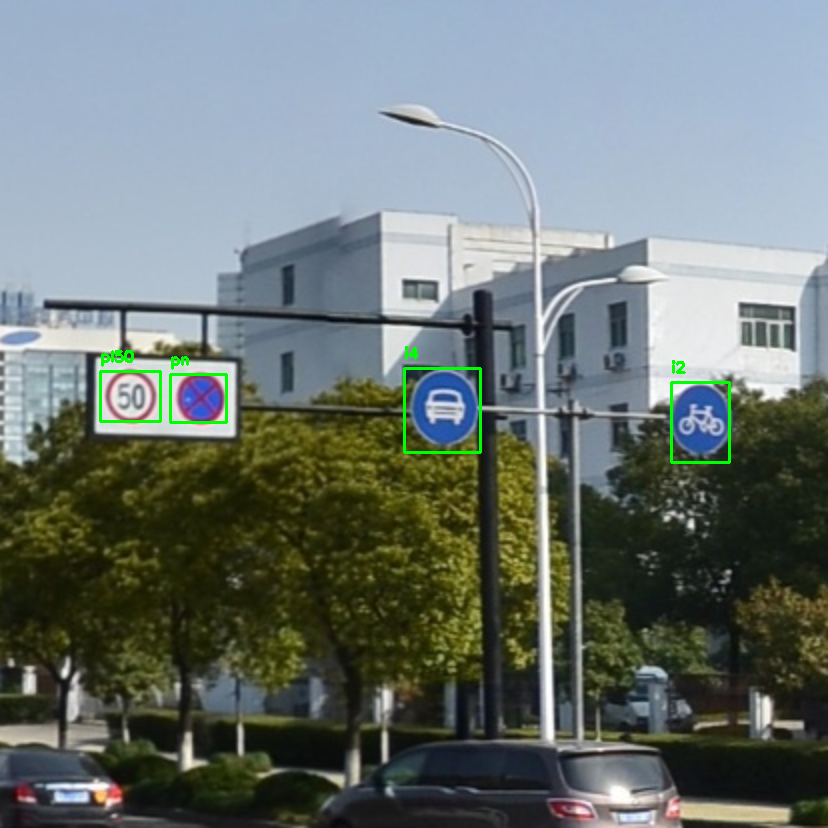
\includegraphics[width=0.48\textwidth]{images/dataset0-enlarged.png}
            \caption{Example image 1}
        \end{subfigure}
        \vspace{0.2cm}
        \begin{subfigure}{\textwidth}
            \centering
            \includegraphics[width=0.48\textwidth]{images/dataset1.png}
            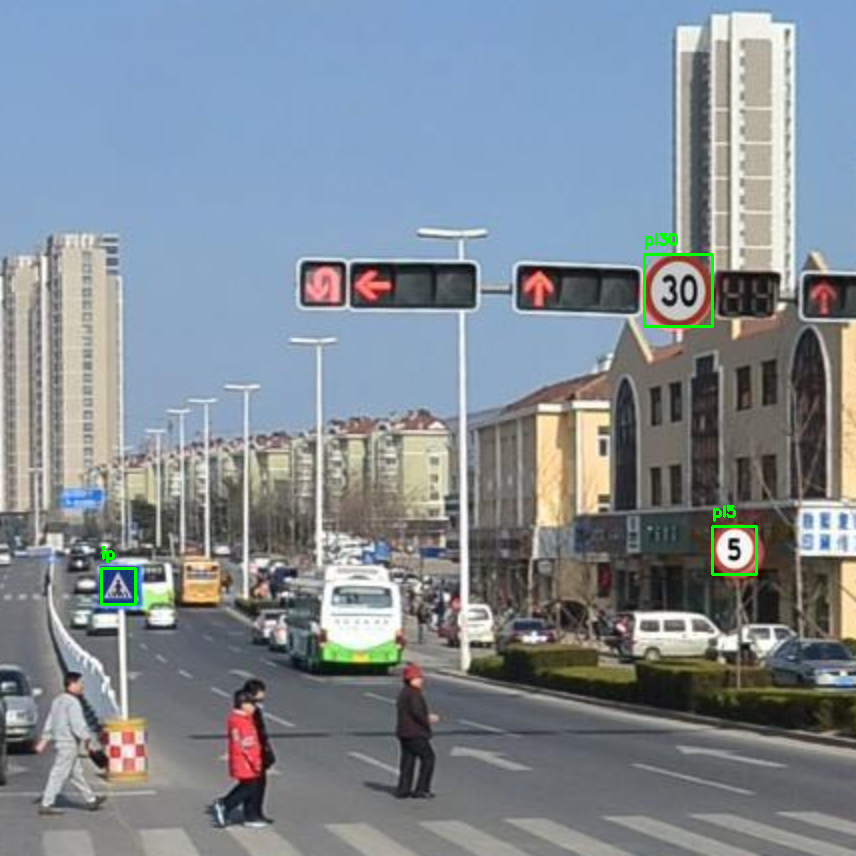
\includegraphics[width=0.48\textwidth]{images/dataset1-enlarged.png}
            \caption{Example image 2}
        \end{subfigure}
        \caption{Examples from TT100K dataset}
        \label{fig:examples}
    \end{minipage}
    \hfill
    \begin{minipage}{0.5\textwidth}
        \centering
        \begin{tabular}{lc}
            \toprule
            Metric & Value \\
            \midrule
            Total Images & 24,052 \\
            Training Images & 20,454 \\
            Validation Images & 3,598 \\
            Total Objects & 74,008 \\
            Training Objects & 63,185 \\
            Validation Objects & 10,823 \\
            Number of Categories & 50 \\
            Train/Val Ratio & 5.84 \\
            Mean Width & 45.5 \\
            Mean Height & 49.4 \\
            Mean Area & 3191.5 \\
            Image Size & 2048x2048 \\
            \bottomrule
        \end{tabular}
        \captionof{table}{Dataset Statistics}
        \label{tab:dataset_stats}
    \end{minipage}
\end{figure}

\begin{figure}[H]
    \centering
    \begin{subfigure}{0.32\textwidth}
        \centering
        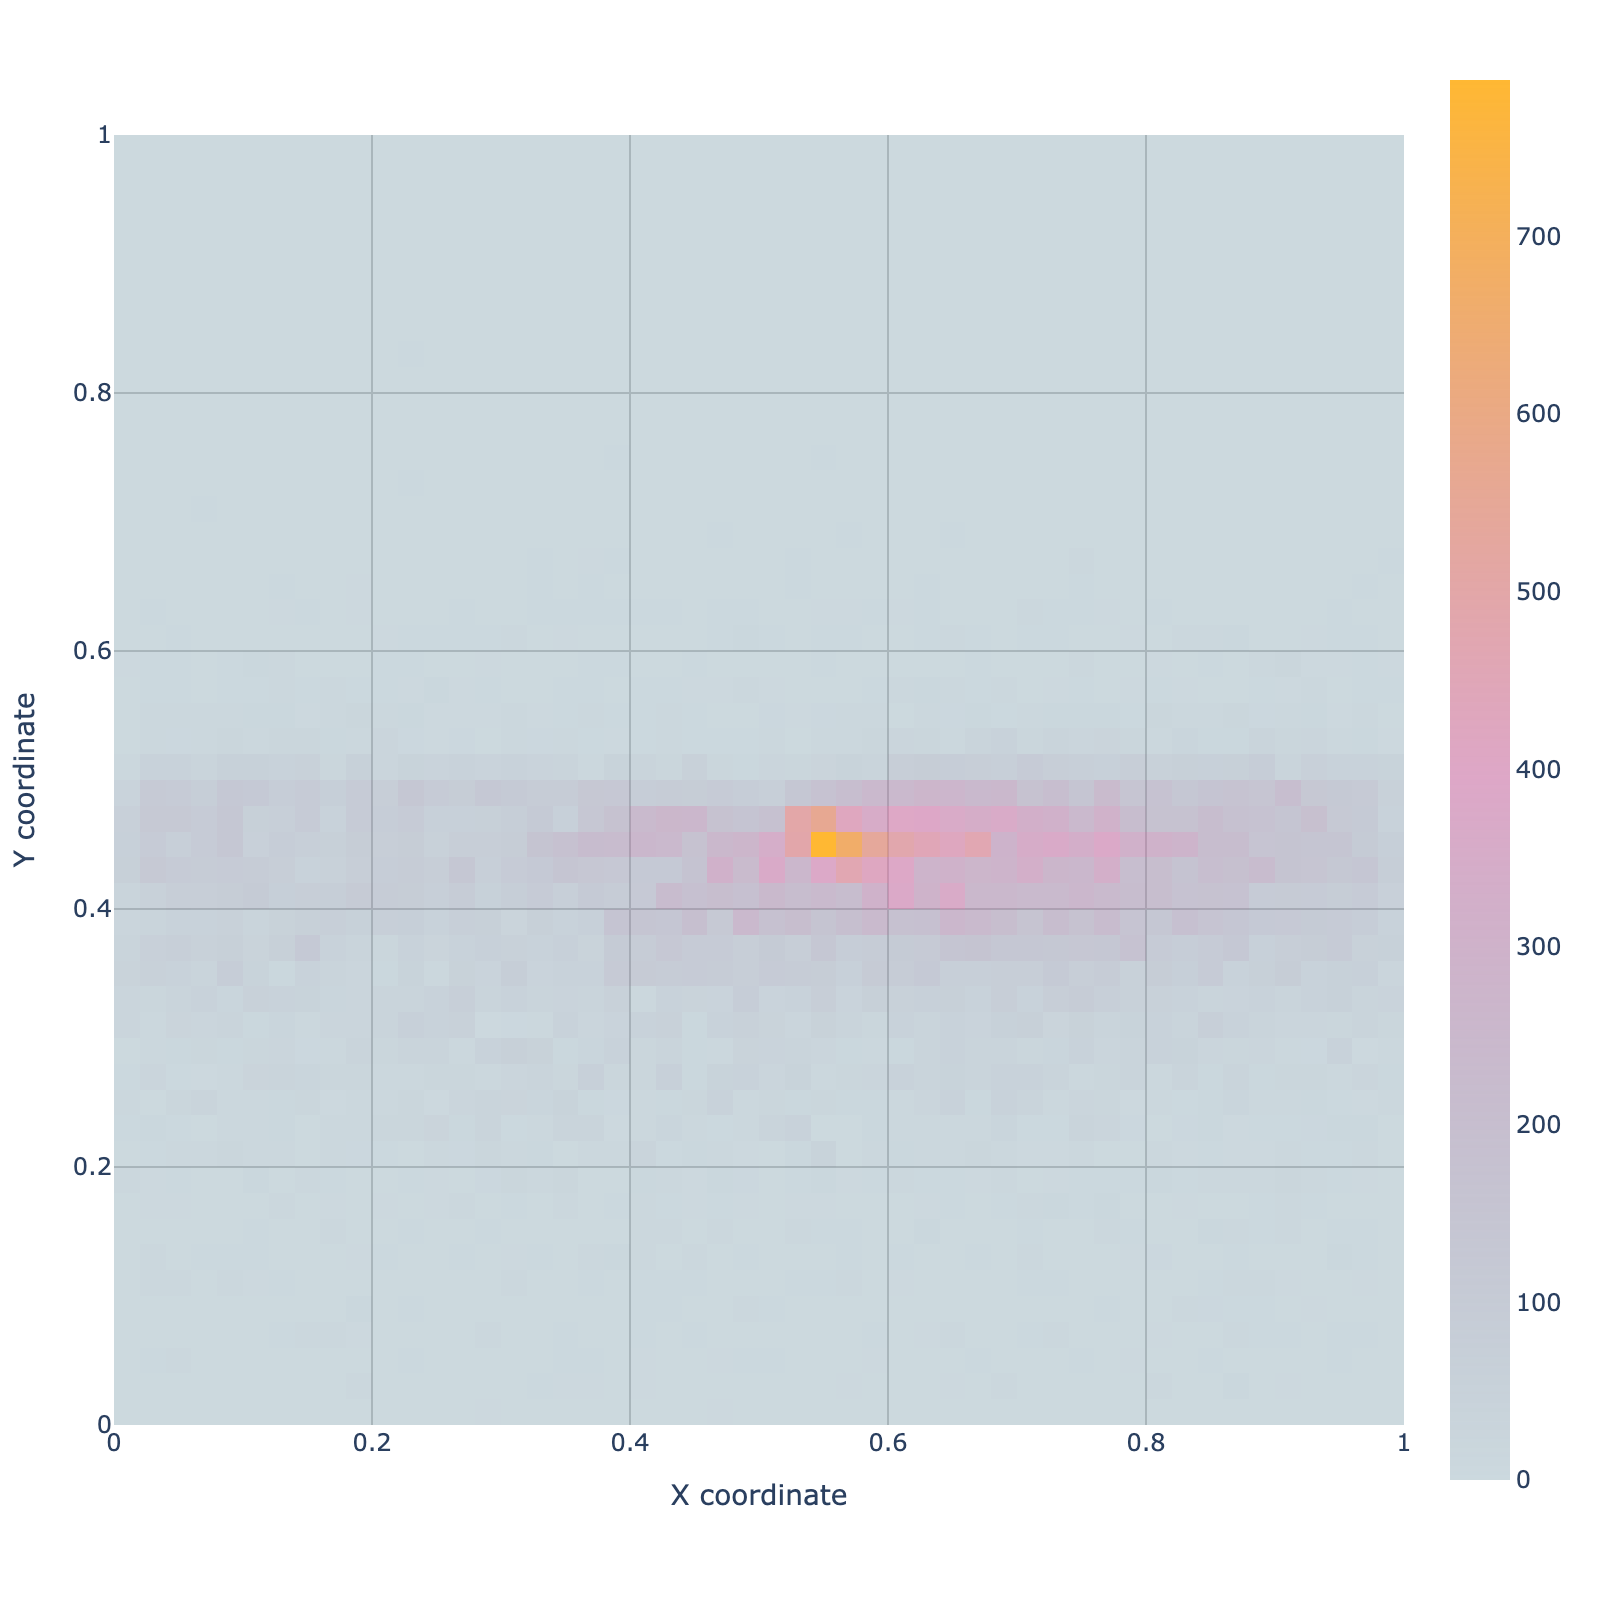
\includegraphics[width=\textwidth]{analysis_results/figures/spatial_distribution.png}
        \caption{Spatial distribution}
        \label{fig:spatial_distribution}
    \end{subfigure}
    \hfill
    \begin{subfigure}{0.32\textwidth}
        \centering
        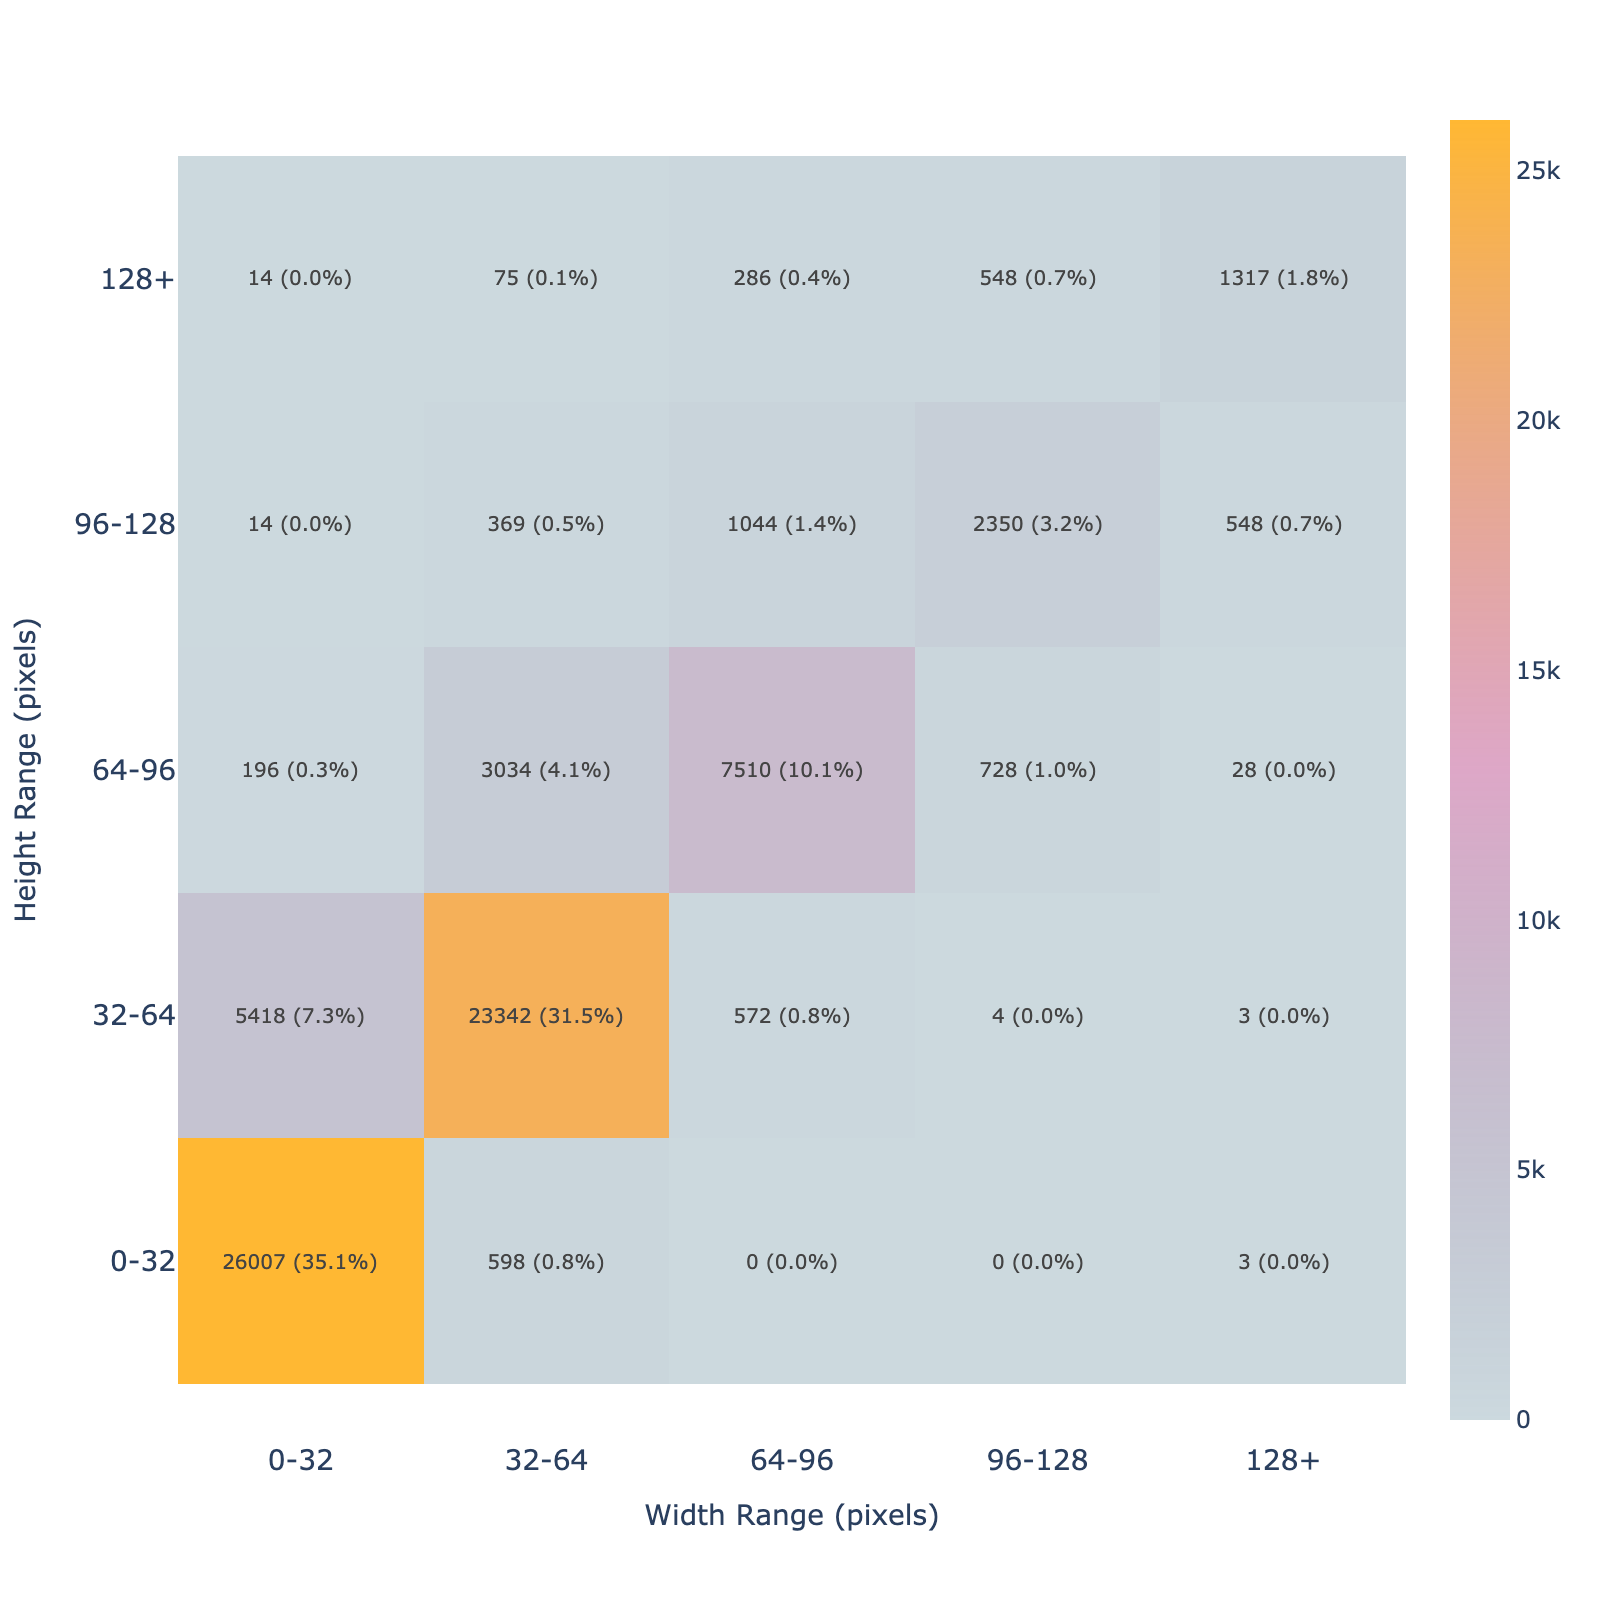
\includegraphics[width=\textwidth]{analysis_results/figures/size_distribution_matrix.png}
        \caption{Size distribution}
    \end{subfigure}
    \hfill
    \begin{subfigure}{0.32\textwidth}
        \centering
        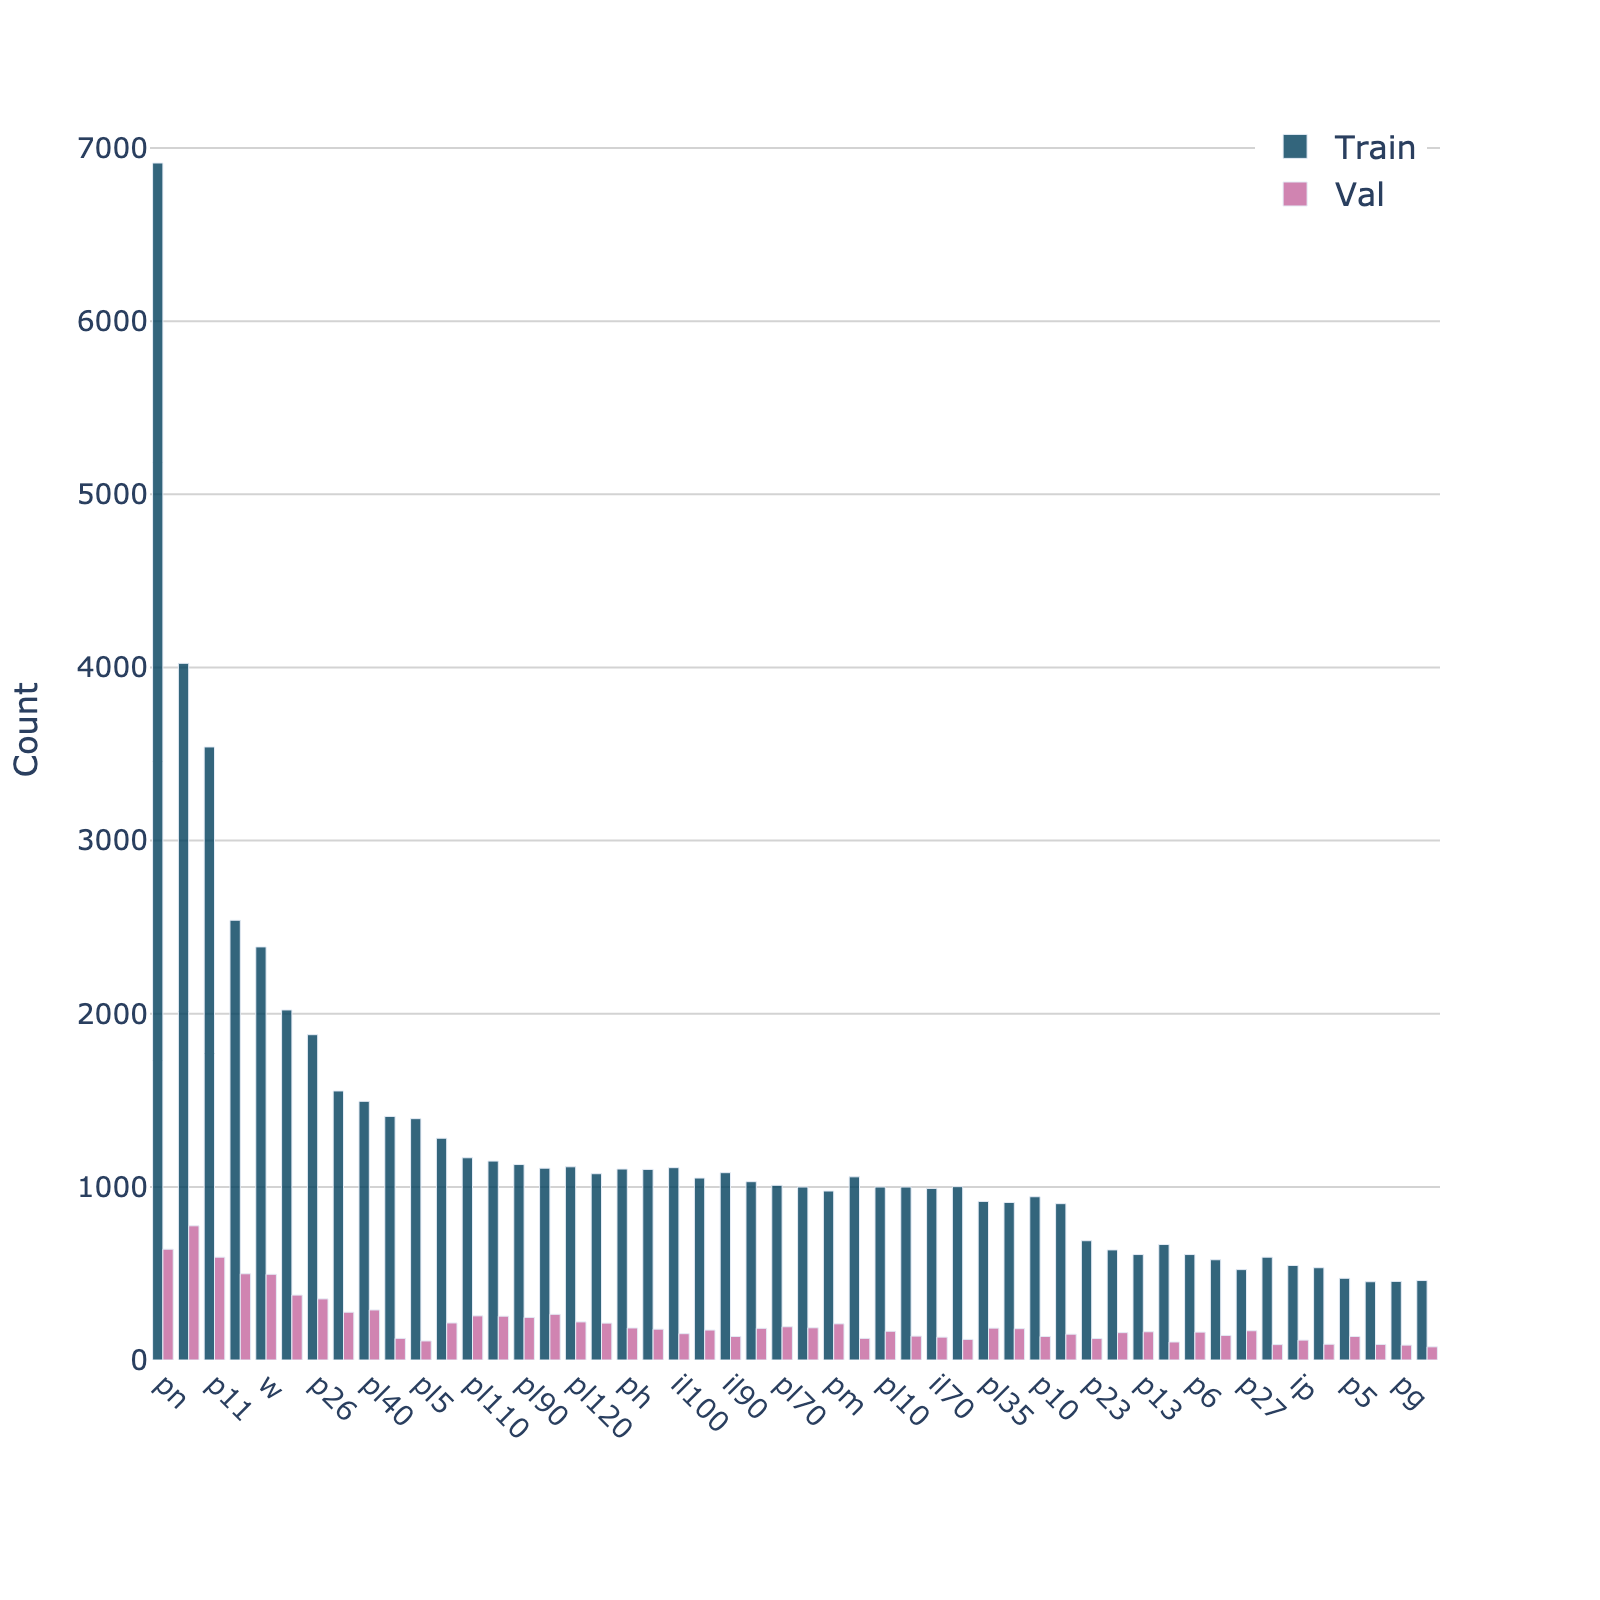
\includegraphics[width=\textwidth]{analysis_results/figures/category_distribution.png}
        \caption{Category distribution}
    \end{subfigure}
    \caption{Distribution analysis of TT100K dataset}
    \label{fig:distributions}
\end{figure}

\subsection{Augmentation}
The normal augmentation methods used in researches can be divided into two categories: \textbf{Basic Augmentations} and \textbf{Advanced Augmentations}.
\begin{small}
\begin{itemize}[leftmargin=*,nosep]
\item \textbf{Basic Augmentations}:
    \begin{itemize}[nosep]
    \item Non-Geometric: Flip, Crop, Color, Noise, Kernel
    \item Geometric: Rotate, Translate, Shear 
    \item Erasing: Random, Hide-and-Seek, GridMask
    \end{itemize}
\item \textbf{Advanced Augmentations}:
    \begin{itemize}[nosep] 
    \item Multi-Image Mixing: Mixup, CutMix, SaliencyMix
    \item Single Image Mixing: Local Aug, Self-Aug
    \item Auto Augment: Random/ADA, RL-based
    \item Feature Level: Feature Space Aug, Style Transfer
    \end{itemize}
\end{itemize}
\end{small}

\section{Methods}
\subsection{YOLO}
YOLO series is a one-stage end-to-end SOTA object detection network. Since the first YOLO was published, it has been the SOTA model among the object detection models. With the help of many computer vision researchers, the YOLO family has been upgrading to YOLOv11 \cite{jocher2024yolo11} published in Sep 2024. For now, the YOLO network mainly consists of 3 parts, Backbone, Neck, and Detection Head(Fig. \ref{fig:yolo_structure}). Figure \ref{fig:yolo_performance} shows the performance of different YOLO models.


\subsection{Global Attention Module}
Attention mechanism is a key component in deep learning now, it enables models to focus on relevant features and ignore irrelevant ones by assigning different weights to different features. In this research, we used two Global Attention Module (GAM) that integrates global information into the YOLO model. GAM enhances feature representation capabilities by introducing channel attention and multi-scale spatial attention mechanisms. For a given input feature map $F \in \mathbb{R}^{C \times H \times W}$, GAM first uses the channel attention sub-module to calculate importance weights $M_c \in \mathbb{R}^{C \times 1 \times 1}$ for each channel, then uses the spatial attention sub-module to calculate importance weights $M_s \in \mathbb{R}^{1 \times H \times W}$ for different spatial positions. The final output feature map $F''$ can be expressed as:
\begin{align}
  F' &= M_c(F) \otimes F \\
  F'' &= M_s(F') \otimes F'
  \label{eq:gam_formula}
\end{align}
where $\otimes$ represents element-wise multiplication.

  \begin{figure}[H]
    \centering
    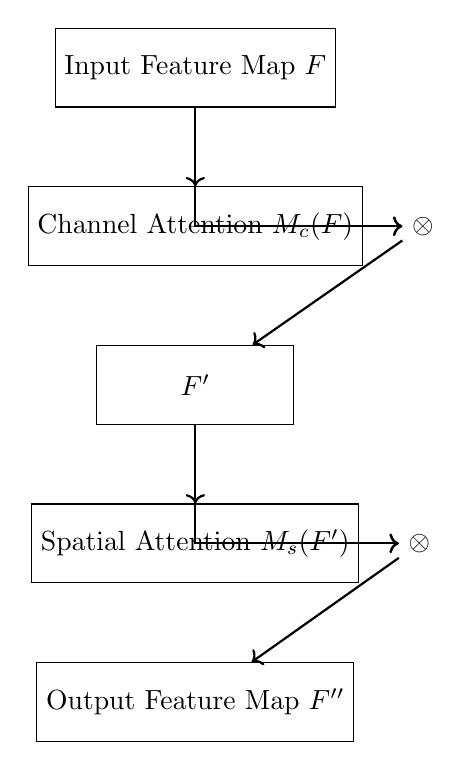
\begin{tikzpicture}[
        block/.style={rectangle, draw, minimum width=2.5cm, minimum height=1cm},
        arrow/.style={->, thick}
    ]
    % Input node
    \node[block] (input) {Input Feature Map $F$};
    
    % Channel attention branch
    \node[block, below=1cm of input] (channel_attention) {Channel Attention $M_c(F)$};
    \node[right=0.5cm of channel_attention] (mul1) {$\otimes$};
    
    % First intermediate feature
    \node[block, below=1cm of channel_attention] (f_prime) {$F'$};
    
    % Spatial attention branch  
    \node[block, below=1cm of f_prime] (spatial_attention) {Spatial Attention $M_s(F')$};
    \node[right=0.5cm of spatial_attention] (mul2) {$\otimes$};
    
    % Output node
    \node[block, below=1cm of spatial_attention] (output) {Output Feature Map $F''$};

    % Connect everything
    \draw[arrow] (input) -- (channel_attention);
    \draw[arrow] (input) |- (mul1);
    \draw[arrow] (channel_attention) -- (mul1);
    \draw[arrow] (mul1) -- (f_prime);
    \draw[arrow] (f_prime) -- (spatial_attention);
    \draw[arrow] (f_prime) |- (mul2);
    \draw[arrow] (spatial_attention) -- (mul2);
    \draw[arrow] (mul2) -- (output);
    \end{tikzpicture}
    \caption{Global Attention Module (GAM) Structure}
    \label{fig:gam_structure}
  \end{figure}
 Compared with Convolutional Block Attention Module(CBAM), GAM can capture more global information and improve the detection accuracy of small objects.
The sequential architecture of GAM(Fig. \ref{fig:cbamandgam}) demonstrates superior efficiency by reducing computational overhead while maintaining detection accuracy. When combined with P2/3/4 detection heads, its hierarchical processing better preserves fine-grained spatial information critical for small objects. Additionally, the streamlined memory footprint makes it particularly suitable for edge deployment scenarios.
\begin{figure}[H]
    \centering
    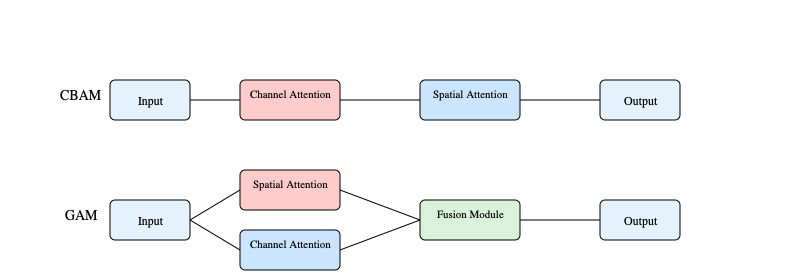
\includegraphics[width=0.8\textwidth]{images/cbamandgam.png}
    \caption{CBAM vs GAM}
    \label{fig:cbamandgam}
\end{figure}

\subsection{SPP family}
The SPP (Spatial Pyramid Pooling)(\ref{fig:spp}) module performs pooling operations on feature maps using different sized pooling kernels and concatenates the results to obtain multi-scale feature representations. For an input feature map $X$, the output $Y$ of SPP can be expressed as:

\begin{equation}
  Y = \text{Concat}(\text{MaxPool}(X, k_1), \text{MaxPool}(X, k_2), ..., \text{MaxPool}(X, k_n))
  \label{eq:spp}
\end{equation}

\begin{figure}[H]
    \centering
    \begin{subfigure}[b]{0.32\textwidth}
        \centering
        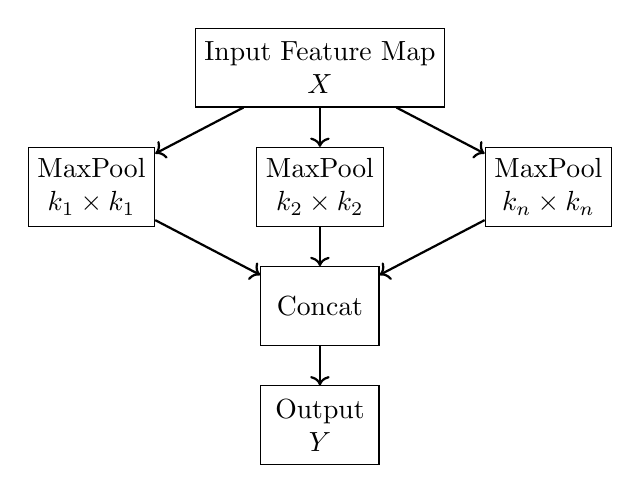
\begin{tikzpicture}[
            scale=0.6,
            block/.style={rectangle, draw, minimum width=1.5cm, minimum height=1cm, align=center},
            arrow/.style={->, thick}
        ]
        \node[block] (input) {Input Feature Map \\ $X$};
        \node[block, below left=0.5cm and 0.5cm of input] (pool1) {MaxPool \\ $k_1 \times k_1$};
        \node[block, below=0.5cm of input] (pool2) {MaxPool \\ $k_2 \times k_2$};
        \node[block, below right=0.5cm and 0.5cm of input] (pool3) {MaxPool \\ $k_n \times k_n$};
        \node[block, below=0.5cm of pool2] (concat) {Concat};
        \node[block, below=0.5cm of concat] (output) {Output \\ $Y$};

        \draw[arrow] (input) -- (pool1);
        \draw[arrow] (input) -- (pool2);
        \draw[arrow] (input) -- (pool3);
        \draw[arrow] (pool1) -- (concat);
        \draw[arrow] (pool2) -- (concat);
        \draw[arrow] (pool3) -- (concat);
        \draw[arrow] (concat) -- (output);
        \end{tikzpicture}
        \caption{SPP Module}
        \label{fig:spp}
    \end{subfigure}
    \hfill
    \begin{subfigure}[b]{0.32\textwidth}
        \centering
        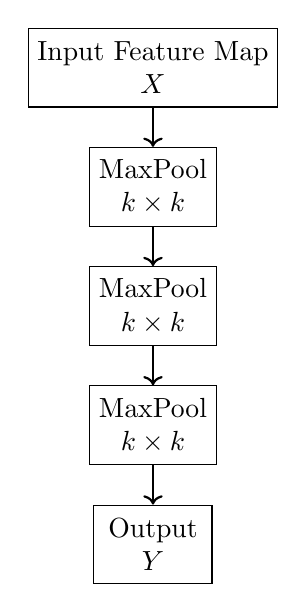
\begin{tikzpicture}[
            scale=0.7,
            block/.style={rectangle, draw, minimum width=1.5cm, minimum height=1cm, align=center},
            arrow/.style={->, thick}
        ]
        \node[block] (input) {Input Feature Map \\ $X$};
        \node[block, below=0.5cm of input] (pool1) {MaxPool \\ $k \times k$};
        \node[block, below=0.5cm of pool1] (pool2) {MaxPool \\ $k \times k$};
        \node[block, below=0.5cm of pool2] (pool3) {MaxPool \\ $k \times k$};
        \node[block, below=0.5cm of pool3] (output) {Output \\ $Y$};
        \draw[arrow] (input) -- (pool1);
        \draw[arrow] (pool1) -- (pool2);
        \draw[arrow] (pool2) -- (pool3);
        \draw[arrow] (pool3) -- (output);
        \end{tikzpicture}
        \caption{SPPF Module}
        \label{fig:sppf}
    \end{subfigure}
    \hfill
    \begin{subfigure}[b]{0.32\textwidth}
        \centering
        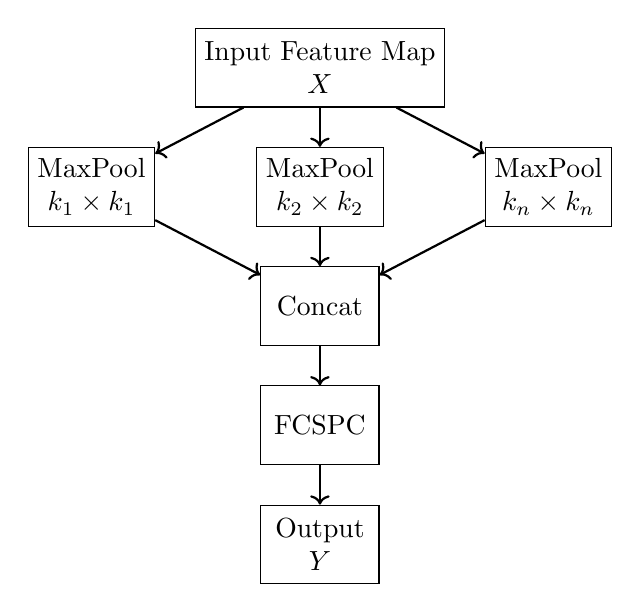
\begin{tikzpicture}[
            scale=0.6,
            block/.style={rectangle, draw, minimum width=1.5cm, minimum height=1cm, align=center},
            arrow/.style={->, thick}
        ]
        \node[block] (input) {Input Feature Map \\ $X$};
        \node[block, below left=0.5cm and 0.5cm of input] (pool1) {MaxPool \\ $k_1 \times k_1$};
        \node[block, below=0.5cm of input] (pool2) {MaxPool \\ $k_2 \times k_2$};
        \node[block, below right=0.5cm and 0.5cm of input] (pool3) {MaxPool \\ $k_n \times k_n$};
        \node[block, below=0.5cm of pool2] (concat) {Concat};
        \node[block, below=0.5cm of concat] (fcspc) {FCSPC};
        \node[block, below=0.5cm of fcspc] (output) {Output \\ $Y$};

        \draw[arrow] (input) -- (pool1);
        \draw[arrow] (input) -- (pool2);
        \draw[arrow] (input) -- (pool3);
        \draw[arrow] (pool1) -- (concat);
        \draw[arrow] (pool2) -- (concat);
        \draw[arrow] (pool3) -- (concat);
        \draw[arrow] (concat) -- (fcspc);
        \draw[arrow] (fcspc) -- (output);
        \end{tikzpicture}
        \caption{SPPFCSPC Module}
        \label{fig:sppfcspc}
    \end{subfigure}
    \caption{Comparison of different SPP modules}
    \label{fig:spp_family}
\end{figure}
SPPF (Spatial Pyramid Pooling - Fast) (\ref{fig:sppf}) is an improved version of SPP that reduces computational cost and increases speed by using multiple cascaded small-sized pooling kernels instead of the large pooling kernels in SPP.
For a given input feature map $X$, the output $Y$ of SPPF can be expressed as:
\begin{equation}
  Y = \text{MaxPool}(\text{MaxPool}(\text{MaxPool}(X, k),k), k)
  \label{eq:sppf}
\end{equation}

SPPFCSPC (Spatial Pyramid Pooling - Fully Connected Spatial Pyramid Convolution) (\ref{fig:sppfcspc}) combines SPP with Fully Connected Spatial Pyramid Convolution (FCSPC) to enhance the network's ability to extract features of different scales and effectively mitigate the impact of object scale variations caused by different factors such as shooting angles and image segmentation.
The expression can be written as:
\begin{equation}
  Y = \text{FCSPC}(\text{Concat}(\text{MaxPool}(X, k_1), \text{MaxPool}(X, k_2), ..., \text{MaxPool}(X, k_n)))
  \label{eq:sppfcspc}
\end{equation}

\subsection{Pruning}
Pruning is a compression technique that compresses a model by removing channels that contribute little to feature extraction in a neural network, with the goal of reducing computational resource consumption (reduce GFLOPS) and model size (reduce model parameters) while maintaining model performance. In this research, we use a pruning method called LAMP (LAYER-ADAPTIVE SPARSITY FOR THE
MAGNITUDE-BASED PRUNING
) \cite{lee2021}, which determines the pruning order by calculating the relative importance score of each weight (weight squared divided by the sum of the squares of all surviving weights in the layer (Eq. \ref{eq:lamp})). After the pruning weight files were obtained, map, precision and recall of the model were reduced, and these important metrics were improved again by fine-tuning. 
\begin{equation}
    \text{LAMP\_score}(w_i^{(l)}) = |w_i^{(l)}| \sqrt{n_l} \text{ where } n_l \text{ is the number of neurons in layer } l
    \label{eq:lamp}
\end{equation}

\subsection{Quantization}
Quantization is a technique that converts model weights and activation values from floating-point representation to low-bit integer representation. For a given floating-point number $x_{\text{fp32}}$, the process of quantizing it to an INT8 integer $q_{\text{int8}}$ can be expressed as:

   \begin{equation}
     q_{\text{int8}} = \text{round}\left(\text{clip}\left(\frac{x_{\text{fp32}}}{s}, -128, 127\right)\right)
     \label{eq:quantization}
   \end{equation}

   where $s$ is the scaling factor, $\text{clip}(x, a, b)$ represents limiting the value of $x$ to the range $[a, b]$, and $\text{round}(x)$ represents rounding $x$ to the nearest integer. The dequantization process can be expressed as:

   \begin{equation}
     x_{\text{fp32}} = s \cdot q_{\text{int8}}
     \label{eq:dequantization}
   \end{equation}

   The choice of scaling factor $s$ affects the precision and dynamic range of quantization. Common methods include scaling based on maximum absolute value and scaling based on KL divergence\cite{nowak2018relaxation}.
    

\section{Experiment and Analysis}
\subsection{Our Model}

\begin{figure}[H]
    \centering
    \begin{minipage}{0.45\textwidth}
        \centering
        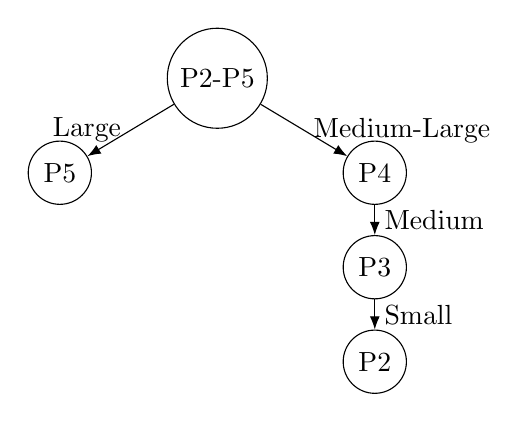
\begin{tikzpicture}[
            scale=0.8,
            level/.style={sibling distance=50mm/#1},
            edge from parent/.style={draw, -{Latex}},
            >=latex
        ]
        \node[circle, draw] (z) {P2-P5}
            child {
                node[circle, draw] (a) {P5} 
                edge from parent node[left] {Large}
            }
            child {
                node[circle, draw] (b) {P4}
                child {
                    node[circle, draw] (c) {P3} 
                    child {
                        node[circle, draw] (d) {P2}
                        edge from parent node[right] {Small}
                    }
                    edge from parent node[right] {Medium}
                }
                edge from parent node[right] {Medium-Large}
            };
        \end{tikzpicture}
        \caption{Feature Pyramid Levels and Object Sizes}
        \label{fig:feature_pyramid}
    \end{minipage}
    \hspace{0.01\textwidth}
    \begin{minipage}{0.40\textwidth}
        \centering
        \caption{Comparison of Models with and without P5 Layer}
        \label{tab:p5_comparison}
        \begin{tabular}{lcccc}
        \toprule
        Model         & Precision & Recall & mAP50 & mAP50-95 \\ \midrule
        With P5       & 0.89641          & 0.80526       & 0.90652      & 0.73618         \\
        Ours & 0.9154           & 0.81115      & 0.91226     & 0.7259        \\ \bottomrule
        \end{tabular}
    \end{minipage}
\end{figure}
In the feature pyramid network (FPN), different layers of feature maps are responsible for detecting objects of different sizes. As shown in Figure \ref{fig:feature_pyramid}, the P2 layer has the highest spatial resolution and is suitable for detecting small objects; the P3 and P4 layers are responsible for detecting medium-sized objects; and the P5 layer has lower spatial resolution and is suitable for detecting large objects. Since the TT100K dataset mainly contains small objects, the P5 layer is limited in its effectiveness, and removing the P5 layer can reduce the model's computational load and improve inference speed, while also avoiding excessive downsampling that leads to loss of small object information. To verify this, we conducted a comparison experiment (Table \ref{tab:p5_comparison}).
Our model (Fig. \ref{fig:yolo—modified}) is a modified YOLOv8s model with GAM attention and P2/3/4 detection heads. It achieves the best performance in all evaluation indicators, among which mAP50 reached 0.91226, an increase of 58.8\% compared with the benchmark model (yolov8s). This result shows the effectiveness of our proposed improved strategy in small object detection tasks. We add two GAM modules, one is after 1st conv layer, and the other is before SPPF-CSPC layer. We also removed the P5 layer and use P2 instead. The features of small objects are more concentrated in the shallow layers, and the features of large objects are more concentrated in the deep layers. So we add two GAM modules to capture the features of small objects and large objects.
Also, we replaced the SPPF with SPPF-CSPC, which is a modified SPPF that uses CSPC instead of C3. CSPC is a new structure that is more suitable for small object detection tasks and faster than SPPF.

\begin{figure}[!h]
    \centering
    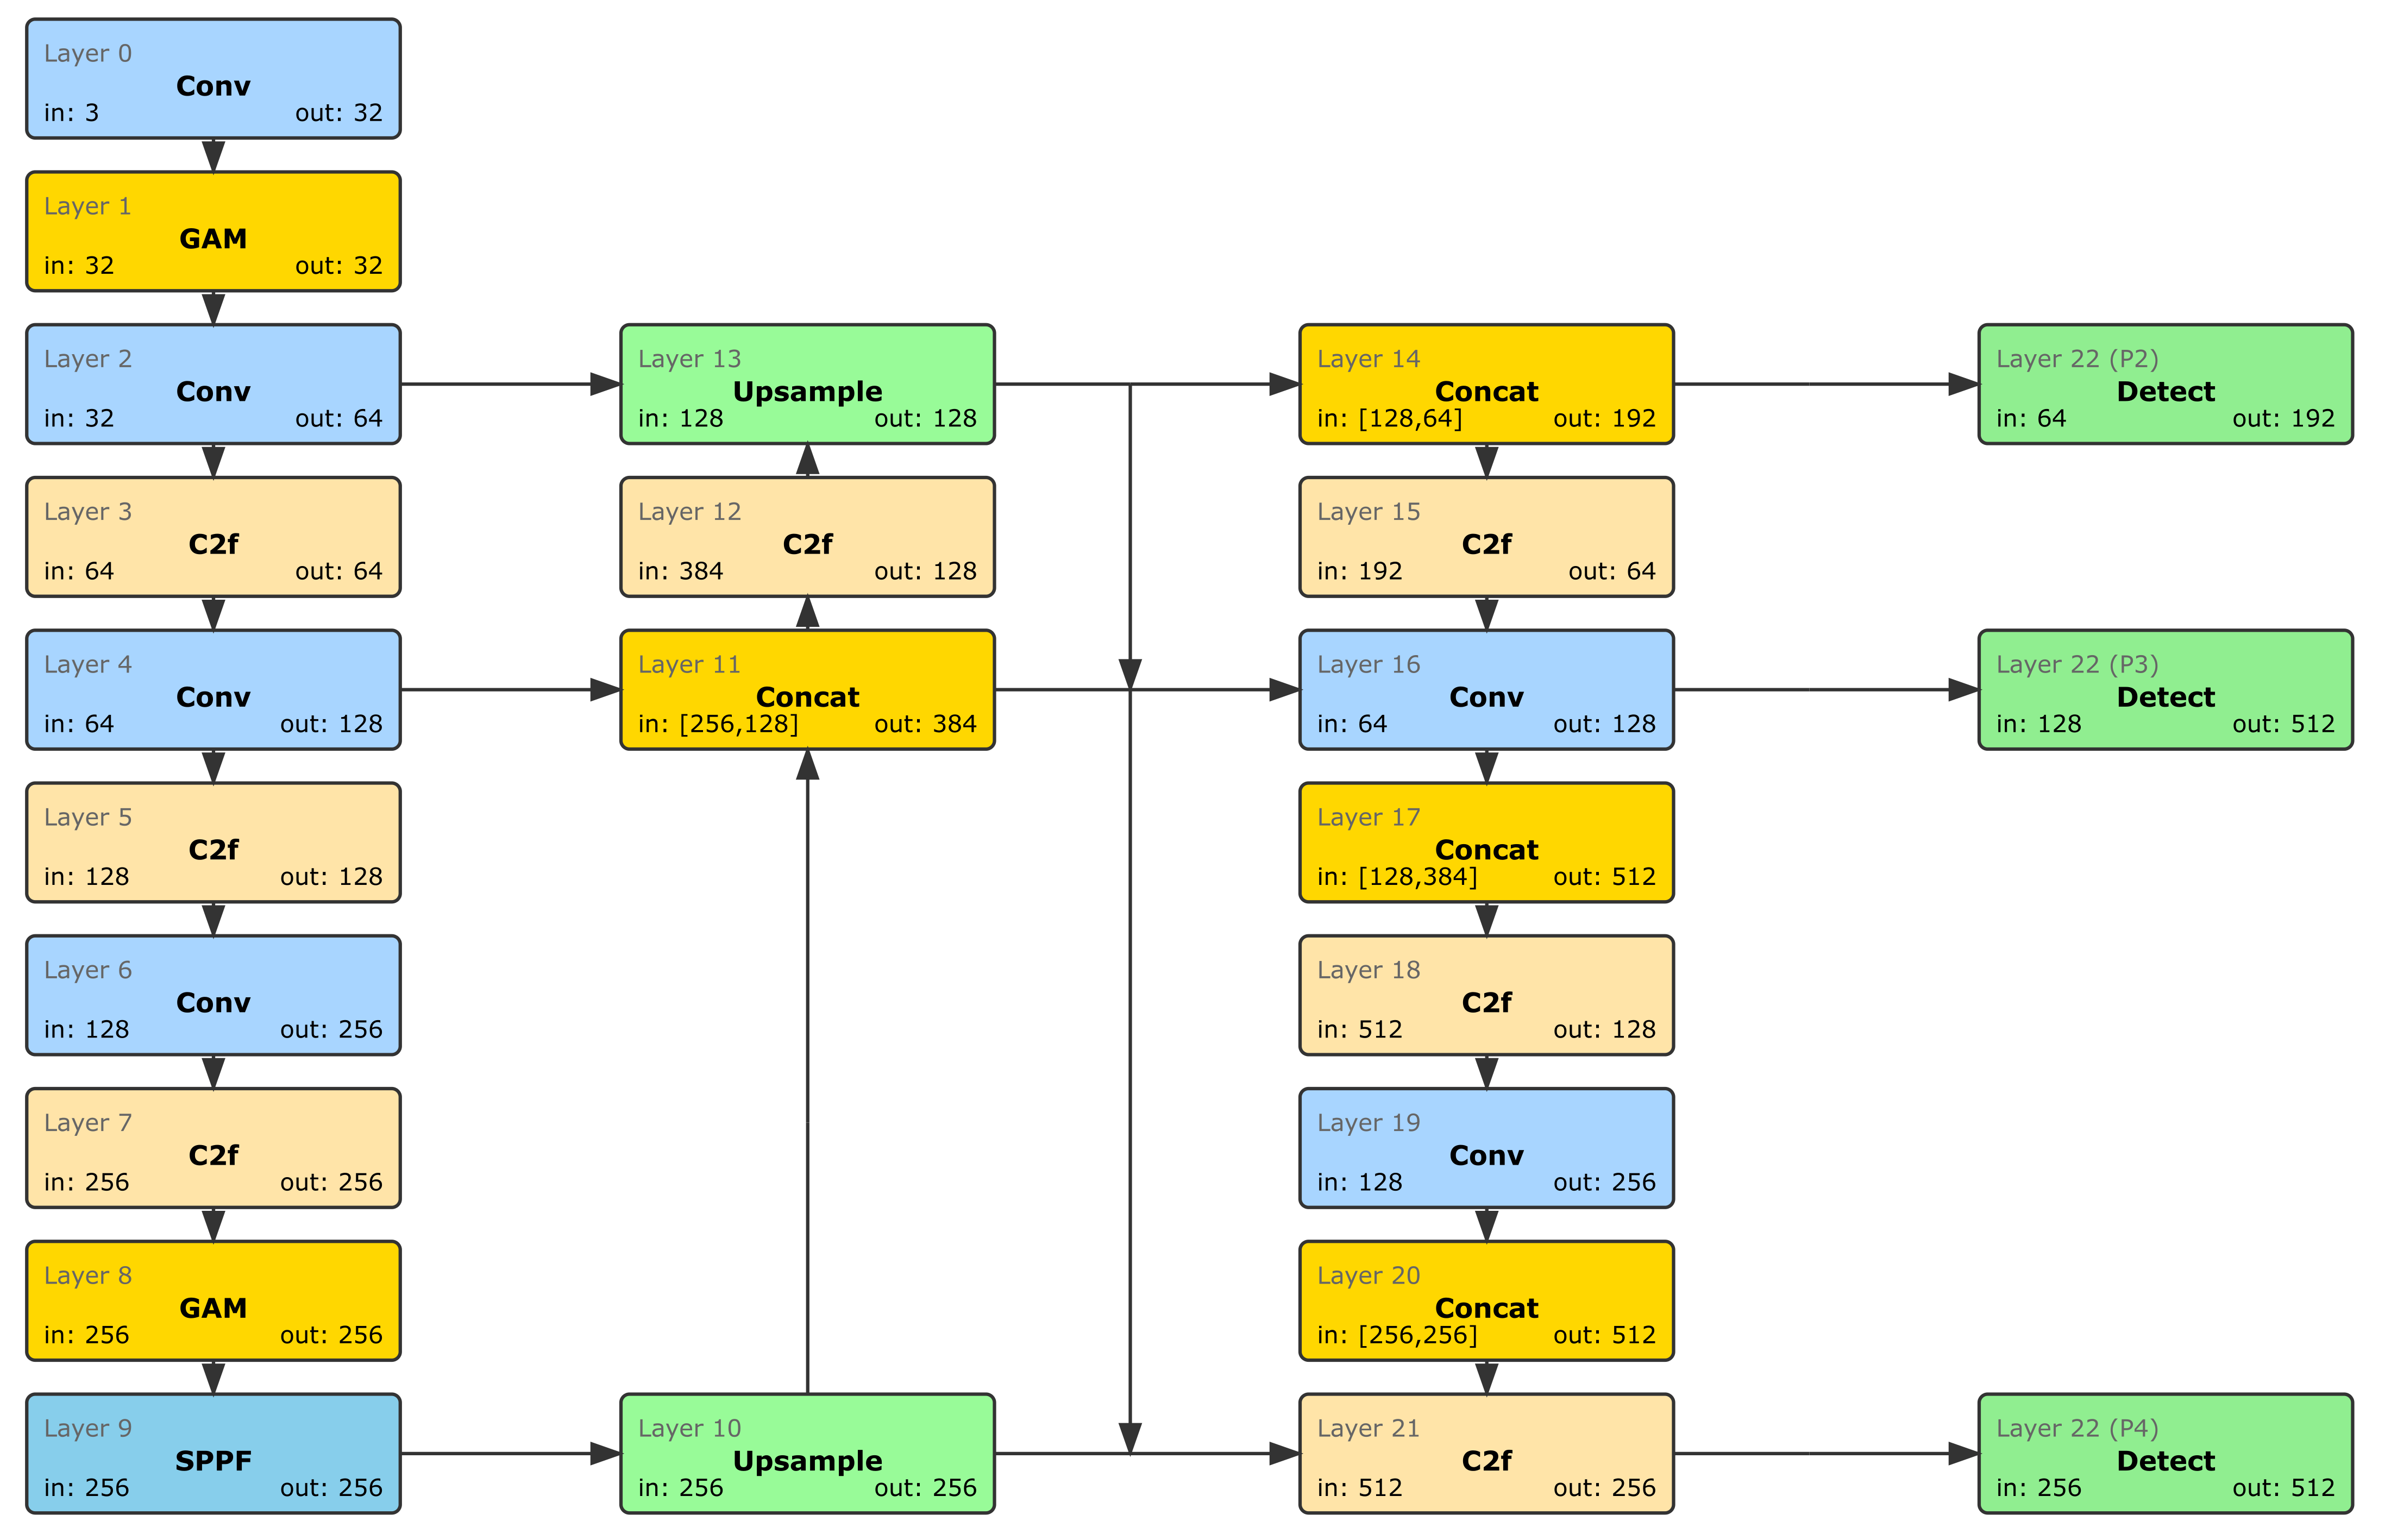
\includegraphics[width=\linewidth]{images/ours.png}
    \caption{Our Modified YOLO with GAM attention and P2/3/4 detection heads}
    \label{fig:yolo—modified}
    \end{figure}
\subsection{YOLO Series Comparison}
\begin{table}[hbtp]
    \centering
    \caption{Performance Comparison: YOLOv8, YOLOv9, and YOLOv10}
    \label{tab:yolov8-v9-v10}
    \begin{tabular}{p{0.16\linewidth}p{0.16\linewidth}p{0.16\linewidth}p{0.16\linewidth}p{0.16\linewidth}}
    \toprule
    Model Name & Precision (B) & Recall (B) & mAP50 (B) & mAP50-95 (B) \\ \midrule
    yolov8s    & 0.65109       & 0.50092    & 0.5777    & 0.46824      \\
    yolov9     & 0.62836       & 0.5042     & 0.57608   & 0.46669      \\
    yolov10s   & 0.58348       & 0.48222    & 0.53559   & 0.43603      \\ \bottomrule
    \end{tabular}
    \end{table}
The comparison of YOLOv8s, YOLOv9, and YOLOv10s reveals relatively similar performance metrics, with YOLOv8s demonstrating a slight edge in overall performance. However, these relatively small differences may become more pronounced in specific application domains, such as small object detection, highlighting the need for further investigation. 

\subsection{Backbone Comparison}
\begin{table}[]
    \centering
    \caption{YOLOv8s Baseline and Lightweight Models for Edge Computing}
    \label{tab:yolov8s-lightweight}
    \begin{tabular}{p{0.16\linewidth}p{0.16\linewidth}p{0.16\linewidth}p{0.16\linewidth}p{0.16\linewidth}}
    \toprule
    Model Name                  & Precision (B) & Recall (B) & mAP50 (B) & mAP50-95 (B) \\ \midrule
    baseline(yolov8s)                     & 0.65109       & 0.50092    & 0.5777    & 0.46824      \\
    FasterNet           & 0.81183       & 0.59062    & 0.71633   & 0.47712      \\
    C2f-GhostBlock            & 0.89491       & 0.76432    & 0.87806   & 0.69342           \\
    MobileNetv4        & 0.81696       & 0.59044    & 0.7147    & 0.51869      \\
    GhostNetv2         & 0.83853       & 0.64894    & 0.77163   & 0.63156      \\
    MobileNeXt-xxs         & 0.72358       & 0.4831     & 0.59016   & 0.31933      \\        
    \textbf{ours}(GAM\_P2/3/4) & \textbf{0.9154} & \textbf{0.81115} & \textbf{0.91226} & \textbf{0.7259} \\
    \bottomrule
    \end{tabular}
    \end{table}

    Table \ref{tab:yolov8s-lightweight} compares several lightweight backbones integrated with YOLOv8s, evaluating their effectiveness for edge computing applications, particularly for small object detection. The baseline model, YOLOv8s, exhibits lower performance metrics than the other models that utilize more efficient backbones. Notably, the C2f-GhostBlock backbone demonstrates significant improvements across all metrics. Our proposed model, incorporating the Global Attention Mechanism (GAM) with a P2/3/4 output layer configuration, achieves superior performance compared to the other models, with the highest precision, recall, mAP50, and mAP50-95 values. These results suggest that our model has considerable potential for accurate and robust small object detection in resource-constrained edge environments.
\subsection{Transformer-based Models}
We also adopt two different light weight transformer based models as backbone, they are Mobilenetv4\cite{mobilenetv4_bottleneck} and EfficientVIT\cite{efficient} . As you can see from the table \ref{tab:transformer-models}, Although their internal network structure also has attention mechanism and feature extraction ability, their performance in detection metric is relatively mediocre.

    \begin{table}[]
        \centering
        \caption{Transformer-based Models: MobileViT and EfficientViT}
        \label{tab:transformer-models}
        \begin{tabular}{p{0.16\linewidth}p{0.16\linewidth}p{0.16\linewidth}p{0.16\linewidth}p{0.16\linewidth}}
        \toprule
        Model Name           & Precision (B) & Recall (B) & mAP50 (B) & mAP50-95 (B) \\ \midrule
        MobileNetv4 & 0.81696       & 0.59044    & 0.7147    & 0.51869      \\
        EfficientViT & 0.73639     & 0.59134   & 0.68897    & 0.55251     \\ \bottomrule
        \end{tabular}
        \end{table}

\subsection{Ablation Experiment}
\begin{table}[]
    \centering
    \caption{Ablation Study with Different Modules}
    \label{tab:gam-ablation}
    \begin{tabular}{p{0.16\linewidth}p{0.16\linewidth}p{0.16\linewidth}p{0.16\linewidth}p{0.16\linewidth}}
    \toprule
    Model Name                  & Precision (B) & Recall (B) & mAP50 (B) & mAP50-95 (B) \\ \midrule
    GAM with SPPF & 0.89641       & 0.80526    & 0.90652   & 0.73618     \\
    singleGAM & 0.90827       & 0.78842    & 0.89547   & 0.7001      \\
    SAM         & 0.89077       & 0.7662     & 0.87621   & 0.67961      \\

    CAM         & 0.90306       & 0.76122    & 0.87979   & 0.69293     \\
    \textbf{ours}        & \textbf{0.9154}        & \textbf{0.81115}    & \textbf{0.91226}   & \textbf{0.7259}       \\
     \bottomrule
    \end{tabular}
    \end{table}
    Table \ref{tab:gam-ablation} and Figure \ref{fig:ablation} present the results of an ablation study investigating the impact of different attention modules and configurations on the performance of our model. Our full model, which incorporates two GAM modules along with the SPPCSPC layer and modified output layers (P2/3/4), achieves the highest overall performance, demonstrating superior precision, recall, mAP50, and mAP50-95. Replacing two GAMs and SPPCSPC with a single GAM and SPPF layer ("GAM with SPPF") results in a slight decrease in precision, recall and mAP50, but a notable increase in mAP50-95. Introducing only a single GAM module to the baseline model ("singleGAM") leads to a more modest drop in overall performance compared to our full model. Replacing the GAM modules with spatial attention ("SAM") or a coordinate attention module across P2/3/4 output layers ("CAM") further diminishes performance across all metrics, particularly mAP50-95. These findings underscore the effectiveness of the GAM module, suggesting that it plays a crucial role in enhancing the model's ability to focus on relevant features and improve detection accuracy. Furthermore, the superior performance of our full model suggests a synergistic effect between using two GAMs and the SPPCSPC, and removing P5 enhances performance.
% At first, we compares the performance of multiple lightweight backbone networks in TT100K. We adapt different types of lightweight models as backbone and use them compared with YOLO owned backbone. EfficientViT achieves good feature representation and maintains a low computational overhead by attention mechanisms and efficient feature aggregation strategies\cite{liu2023evit}. FasterNet uses an creative feature recombination method that increases the training and inference speed\cite{faster}. Moreover, lightweight networks such as MobileNeXt\cite{mobile} and GhostNet\cite{ghost} achieve a good balance of computational efficiency and performance on edge devices by designing novel lightweight modules. From the experimental results in Table \ref{tab:yolo_performance}, we can see our modified model has achieved remarkable results. The improved model based on GAM attention mechanism (\texttt{yolov8s\_GAM\_smalltarget\_noP5}) achieved the best performance in all evaluation indicators, among which mAP50 reached 0.91226, an increase of 58.8\% compared with the benchmark model (yolov8s). This result shows the effectiveness of our proposed improved strategy in small object detection tasks.

\begin{figure}[!h]
\centering
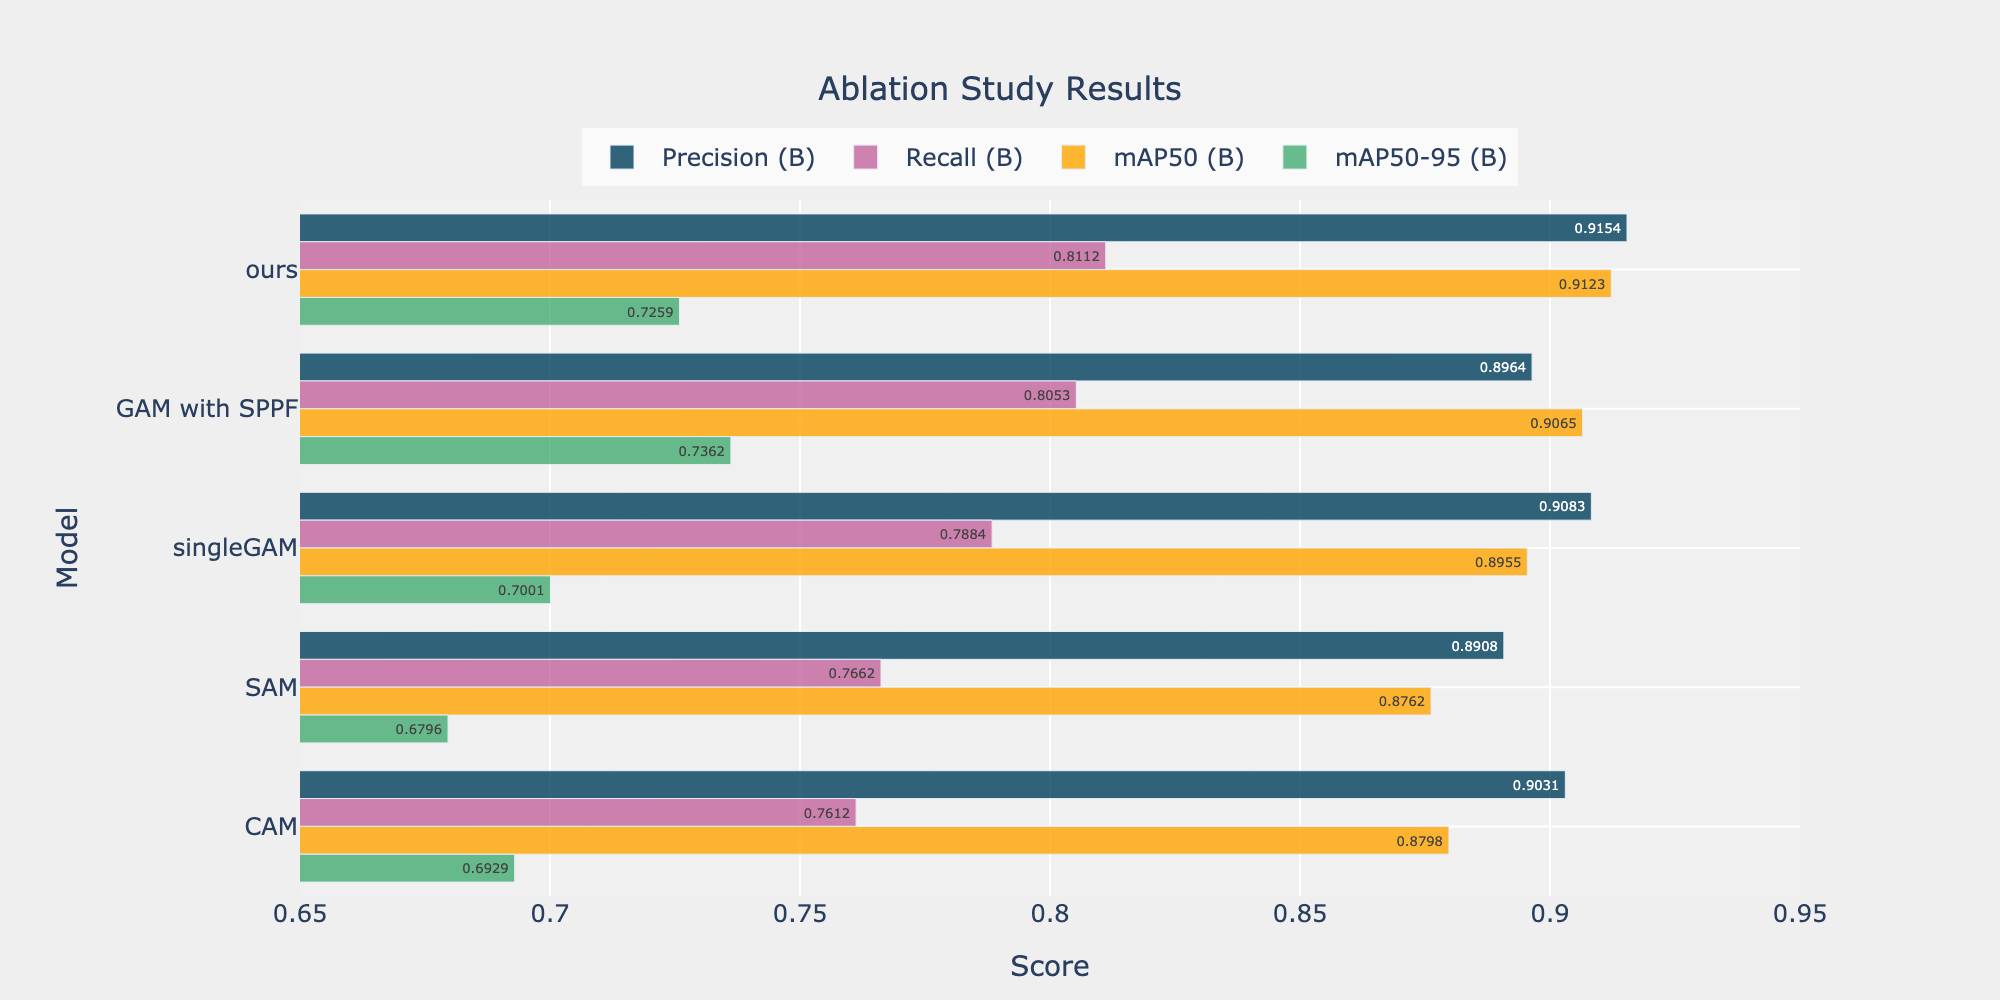
\includegraphics[width=\linewidth]{images/ablation_study.png}
\caption{Ablation Experiment}
\label{fig:ablation}
\end{figure}
In order to further analyze the influence of different modules on the model performance, we studied the contribution of each modification through the control variable method. Therefore, our ablation experiments is conducted as shown in Figure \ref{fig:ablation}

\begin{itemize}

\item \textbf{base (11.17M)} : The original YOLOv8s model as the baseline

\item \textbf{MobileNeXt (7.41M)} : Use lightweight backbone instead

\item \textbf{GAM P2-5 (23.87M)} : Added GAM attention mechanism and P2 detect head

\item \textbf{base with P2-5 (10.86M)} : Adds P2 detect head to the base model

\item \textbf{GAM P2-4 SPPF (11.75M)} : Our complete improvement but keep SPPF

\item \textbf{CBAM\_smalltarget (5.14M)} : A lightweight version that uses the CBAM attention mechanism

\item \textbf{single GAM (8.14M)} : Only a single GAM module is used

\item \textbf{ours (10.01M)} : Our final modification

\end{itemize}


From the experimental results, we can observe that the GAM attention mechanism brings a significant improvement, compared to the original base model, precision improved from 0.65 to 0.87, and mAP50 also improved from 0.58 to 0.85. In terms of detection head optimization, the addition of P2 detection head significantly improves the detection ability of the model for small objects, which can be seen in the base with P2-5 configuration, whose mAP50-95 increases from 0.47 to 0.61.

More importantly, when we removed the P5 detection head, the model not only maintained high performance, but also reduced the number of parameters from 11.7M to 10.01M, and reaches a nice detection metrics where precision 0.92, recall 0.81, mAP50 0.91. For attention mechanism, the experiment proves that GAM has obvious advantages over CBAM. This ablation experiment not only validate the effectiveness of each modification we add, but also demonstrate that the combination of these components leads to an ideal performance improvements, which assists our design decisions for SOD optimization.

\subsection{Model compression}
In Figure \ref{fig:Channel} we compare the number of channels before and after pruning. We can see that in the shallow and middle layers of the network, more channels are pruned. In particular, a large number of channels are eliminated in the conv layers near to the neck. Acording to table \ref{tab:model_compression}, after pruning, our model parameters and GFLOS have been reduced by nearly half from 10M to 5.46M and  from 102.4 to 50.7, which is more suitable for our edge deployment. However, dection metrics including recall, precision and mAP50 only reduced within 1\%. After pruning and quantization, our model inference speed is up to 6 times faster, and the FPS is increased from 104.17 to 666.67. Although pruning plus int8 quantization does the same number of operations as pruning alone, we get a significant speedup compared to floating-point arithmetic because of the int8 type. Honestly, while gaining speed improvement, we also encountered some loss in detection metrics, we sacrificed recal,l precision and mAP50, but these reductions were within 10\%.

\begin{figure}[!h]
\centering
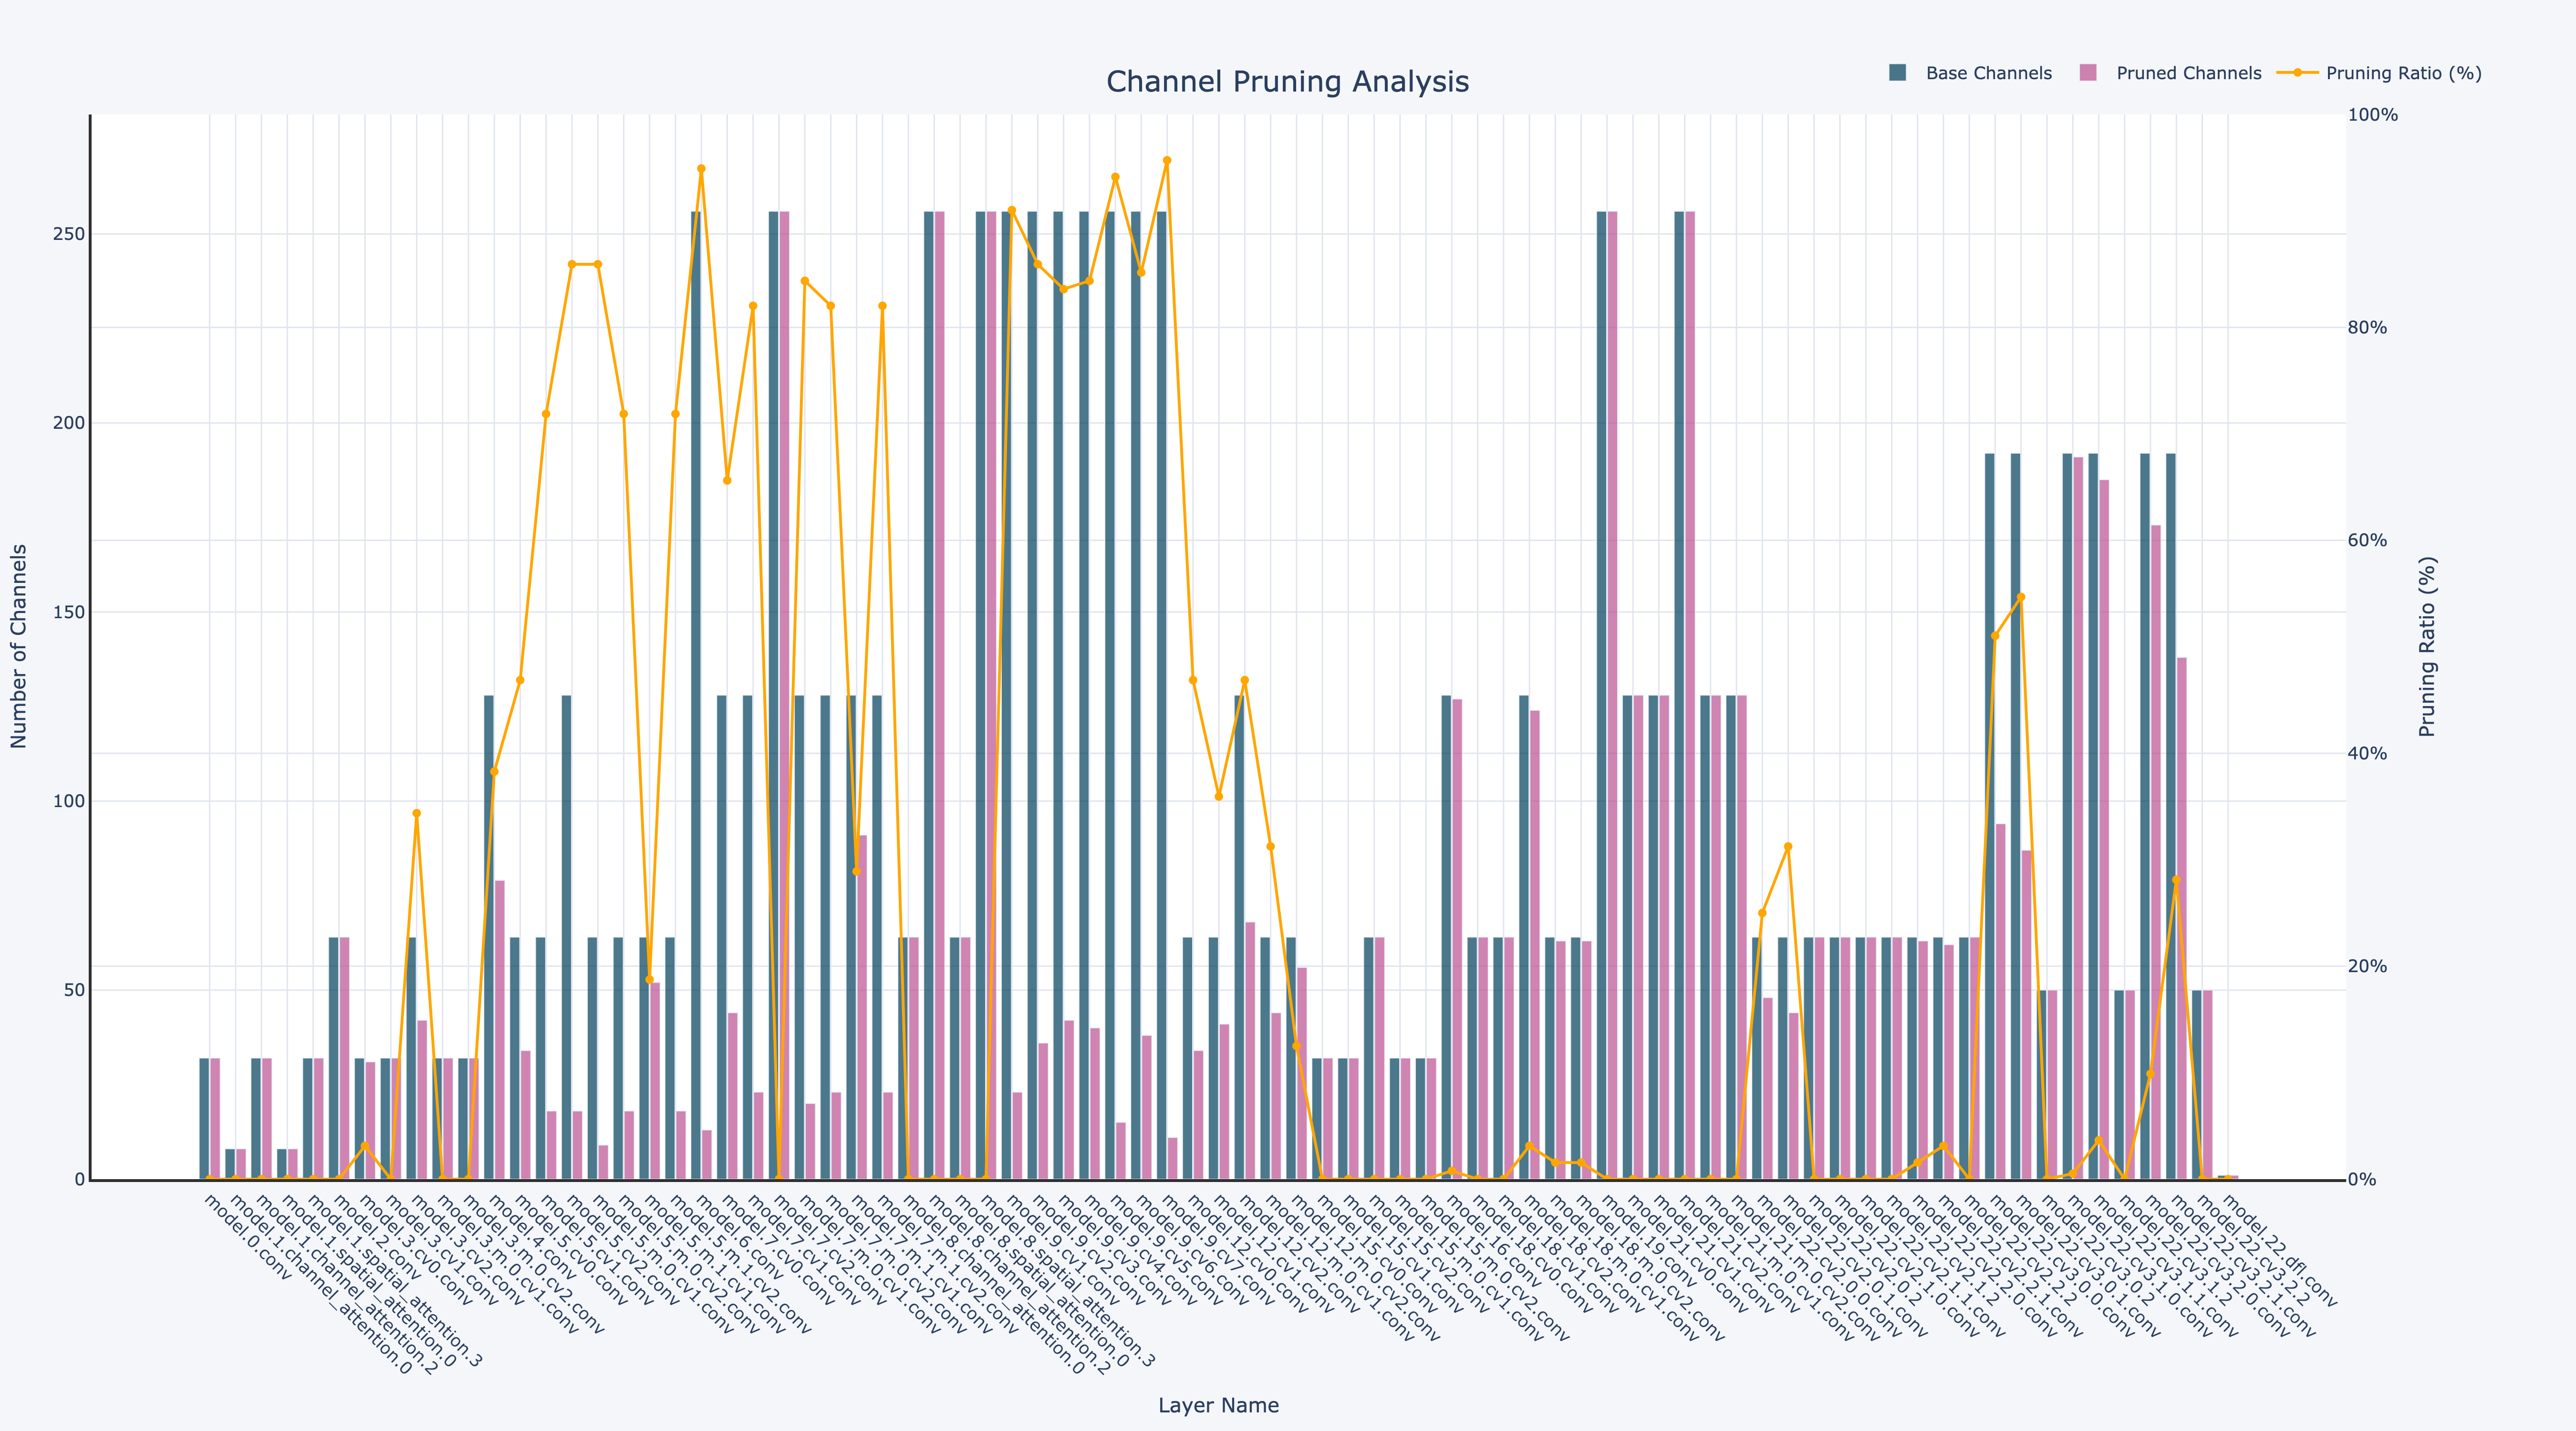
\includegraphics[width=1.0\linewidth]{images/channel.png}
\caption{Channel pruning analysis}
\label{fig:Channel}
\end{figure}

\begin{table}
\centering

\begin{tabular}{p{0.18\linewidth}p{0.15\linewidth}p{0.18\linewidth}p{0.18\linewidth}p{0.22\linewidth}}
    \hline
    Metrics &  & Original & Pruning & Pruning+TensorRT INT8 \\
    \hline
    \multirow{3}{*}{FPS} & V100 & 91.15 & 114.98 & 229.97 \\
     & A10 & 104.17 & 131.87 & 666.67 \\
     & A100 & 117.19 & 148.36 & 853.40 \\
    \hline
    \multicolumn{2}{l}{Parameters (Millions)} & 10.0 & 5.46 & 5.46 \\
    \multicolumn{2}{l}{GFLOPS or GOPS} & 102.4 & 50.7 & 50.7 \\
    \multicolumn{2}{l}{Precision} & 0.91413 & 0.90891 & 0.83381 \\
    \multicolumn{2}{l}{Recall} & 0.81045 & 0.80400 & 0.69251 \\
    \multicolumn{2}{l}{mAP50} & 0.91183 & 0.90552 & 0.82779 \\
    \multicolumn{2}{l}{mAP50-95} & 0.73862 & 0.78170 & 0.68005 \\
    \hline
    \end{tabular}
    \caption{Inference Performance Comparison}
    \label{tab:model_compression}
    \end{table}
\section{Limitations and Discussion}
    While our model achieves strong performance, several limitations should be noted:
    
    1. The model's performance may degrade when dealing with extremely small objects (< 16×16 pixels) or under severe occlusion conditions.
    
    2. The dual GAM modules introduce additional computational overhead, which could be problematic for devices with very limited computational resources.
    
    3. The current pruning strategy is based on magnitude, which may not be optimal for all deployment scenarios. More sophisticated pruning methods could potentially achieve better compression-accuracy trade-offs.
    
    These limitations suggest directions for future research, including developing more efficient attention mechanisms and exploring hardware-aware compression strategies.
\section{Conclusion and Future Work}
This research demonstrates the effectiveness of integrating a Global Attention Module (GAM) and optimizing detection heads (P2/3/4, without P5) within the YOLOv8s architecture for improved small object detection, particularly for traffic signs in the TT100K dataset. Our model achieves state-of-the-art performance, evidenced by a mAP50 of 0.91226. Ablation studies confirm the significant contributions of the dual GAM integration and SPPCSPC layer. Furthermore, model compression via pruning and quantization substantially reduces model size and computational requirements, leading to a significant boost in inference speed (up to sixfold) while maintaining acceptable accuracy. The results underscore the feasibility of deploying advanced deep learning models on edge devices for real-time SOD.

Future work will focus on several key areas:
\begin{enumerate}
    \item \textbf{Model Refinement:} Further refining the model architecture by exploring alternative attention mechanisms and optimizing the balance between accuracy and efficiency.
    \item \textbf{Advanced Data Augmentation:} Investigating advanced data augmentation techniques to enhance model robustness and generalizability across diverse scenarios.
    \item \textbf{Generalization Ability:} Exploring more datasets about traffic object detection and adapt our model to these datasets to improve the generalization ability.
    \item \textbf{Edge Device Deployment:} Evaluating the optimized model's performance on various edge computing devices, including the NVIDIA Orin AGX X, to validate its real-world applicability and efficiency.
    \item \textbf{Tracking New Methods:} Continuously monitoring advancements in image processing and deep learning for potential integration into the SOD pipeline.
\end{enumerate}


%%% Uncomment this section and comment out the \bibliography{references} line above to use inline references.
% \begin{thebibliography}{1}

% 	\bibitem{kour2014real}
% 	George Kour and Raid Saabne.
% 	\newblock Real-time segmentation of on-line handwritten arabic script.
% 	\newblock In {\em Frontiers in Handwriting Recognition (ICFHR), 2014 14th
% 			International Conference on}, pages 417--422. IEEE, 2014.

% 	\bibitem{kour2014fast}
% 	George Kour and Raid Saabne.
% 	\newblock Fast classification of handwritten on-line arabic characters.
% 	\newblock In {\em Soft Computing and Pattern Recognition (SoCPaR), 2014 6th
% 			International Conference of}, pages 312--318. IEEE, 2014.

% 	\bibitem{hadash2018estimate}
% 	Guy Hadash, Einat Kermany, Boaz Carmeli, Ofer Lavi, George Kour, and Alon
% 	Jacovi.
% 	\newblock Estimate and replace: A novel approach to integrating deep neural
% 	networks with existing applications.
% 	\newblock {\em arXiv preprint arXiv:1804.09028}, 2018.

% \end{thebibliography}
\newpage
\printbibliography
\newpage
\appendix
\section{Figures}
\begin{figure}[H]
    \centering
        \centering
        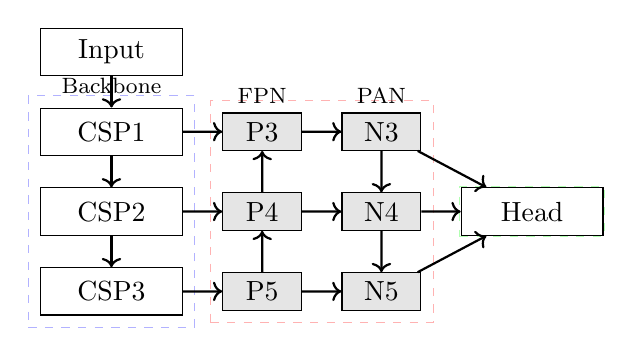
\begin{tikzpicture}[
            scale=1,
            block/.style={rectangle, draw, minimum width=1.8cm, minimum height=0.6cm},
            arrow/.style={->, thick, scale=0.8},
            feature/.style={rectangle, draw, minimum width=1cm, minimum height=0.4cm, fill=gray!20},
            skip/.style={->, dashed, thick}
        ]
        \node[block] (input) at (0,0) {Input};
        \node[block, below=0.4cm of input] (backbone1) {CSP1};
        \node[block, below=0.4cm of backbone1] (backbone2) {CSP2};
        \node[block, below=0.4cm of backbone2] (backbone3) {CSP3};
        \node[feature, right=0.5cm of backbone1] (fpn3) {P3};
        \node[feature, right=0.5cm of backbone2] (fpn2) {P4};
        \node[feature, right=0.5cm of backbone3] (fpn1) {P5};
        \node[feature, right=0.5cm of fpn3] (pan3) {N3};
        \node[feature, right=0.5cm of fpn2] (pan2) {N4};
        \node[feature, right=0.5cm of fpn1] (pan1) {N5};
        \node[block, right=0.5cm of pan2] (head) {Head};
        \draw[arrow] (input) -- (backbone1);
        \draw[arrow] (backbone1) -- (backbone2);
        \draw[arrow] (backbone2) -- (backbone3);
        \draw[arrow] (backbone1) -- (fpn3);
        \draw[arrow] (backbone2) -- (fpn2);
        \draw[arrow] (backbone3) -- (fpn1);
        \draw[arrow] (fpn1) -- (fpn2);
        \draw[arrow] (fpn2) -- (fpn3);
        \draw[arrow] (fpn3) -- (pan3);
        \draw[arrow] (fpn2) -- (pan2);
        \draw[arrow] (fpn1) -- (pan1);
        \draw[arrow] (pan3) -- (pan2);
        \draw[arrow] (pan2) -- (pan1);
        \draw[arrow] (pan3) -- (head);
        \draw[arrow] (pan2) -- (head);
        \draw[arrow] (pan1) -- (head);
        \node[above=0.05cm of backbone1,font=\footnotesize] {Backbone};
        \node[above=1cm of fpn2,font=\footnotesize] {FPN};
        \node[above=1cm of pan2,font=\footnotesize] {PAN};
        \begin{scope}[on background layer]
            \node[fit=(backbone1)(backbone2)(backbone3), draw=blue!30, dashed, inner sep=0.15cm] {};
            \node[fit=(fpn1)(fpn2)(fpn3)(pan1)(pan2)(pan3), draw=red!30, dashed, inner sep=0.15cm] {};
            \node[fit=(head), draw=green!30, dashed, inner sep=0.01cm] {};
        \end{scope}
        \end{tikzpicture}
        \caption{YOLO network architecture}
        \label{fig:yolo_structure}
\end{figure}
\begin{figure}[H]
    \centering
    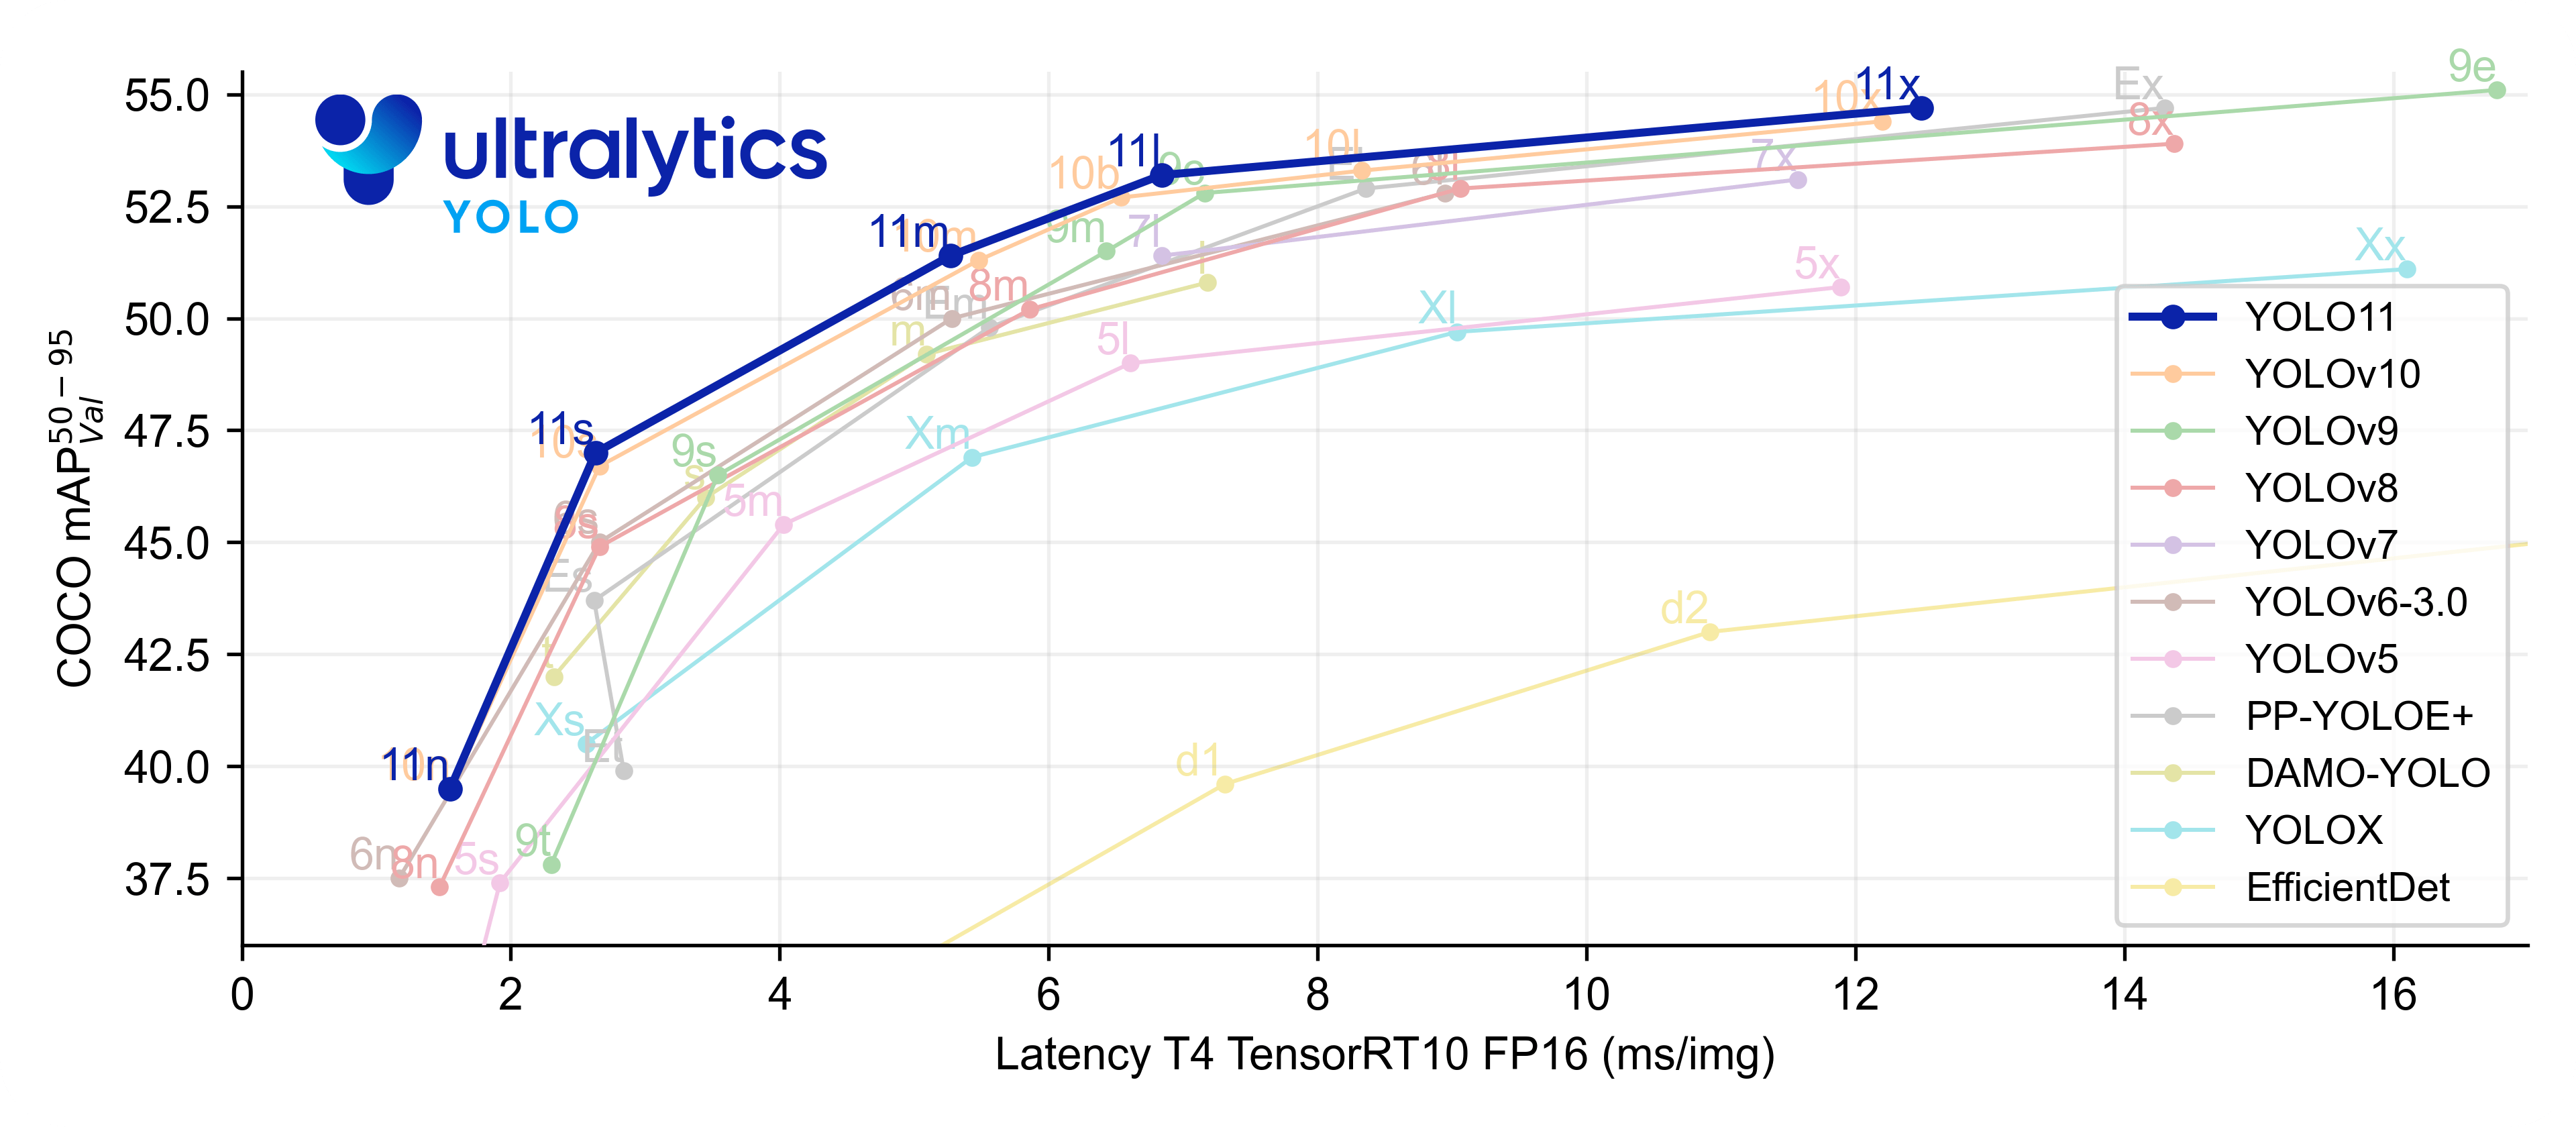
\includegraphics[width=\textwidth]{images/performance-comparison.png}
    \caption{YOLO performance comparison}
    \label{fig:yolo_performance}
\end{figure}
\newpage
\subsection{Appendix 1 - Our Model Yaml Configuration}
\begin{lstlisting}
    # Ultralytics YOLO, AGPL-3.0 license
# YOLOv8 object detection model with P3-P5 outputs. For Usage examples see https://docs.ultralytics.com/tasks/detect

# Parameters
nc: 1  # number of classes
scales: # model compound scaling constants, i.e. 'model=yolov8n.yaml' will call yolov8.yaml with scale 'n'
  # [depth, width, max_channels]
  n: [0.33, 0.25, 1024]  # YOLOv8n summary: 225 layers,  3157200 parameters,  3157184 gradients,   8.9 GFLOPs
  s: [0.33, 0.50, 1024]  # YOLOv8s summary: 225 layers, 11166560 parameters, 11166544 gradients,  28.8 GFLOPs
  m: [0.67, 0.75, 768]   # YOLOv8m summary: 295 layers, 25902640 parameters, 25902624 gradients,  79.3 GFLOPs
  l: [1.00, 1.00, 512]   # YOLOv8l summary: 365 layers, 43691520 parameters, 43691504 gradients, 165.7 GFLOPs
  x: [1.00, 1.25, 512]   # YOLOv8x summary: 365 layers, 68229648 parameters, 68229632 gradients, 258.5 GFLOPs

# YOLOv8.0n backbone
backbone:
   # [from, repeats, module, args]
  - [-1, 1, Conv, [64, 3, 2]]  # 0-P1/2
  - [-1, 1, GAM_Attention, []]
  - [-1, 1, Conv, [128, 3, 2]]  # 1-P2/4
  - [-1, 3, C2f, [128, True]]
  - [-1, 1, Conv, [256, 3, 2]]  # 3-P3/8
  - [-1, 6, C2f, [256, True]]
  - [-1, 1, Conv, [512, 3, 2]]  # 5-P4/16
  - [-1, 6, C2f, [512, True]]
  - [-1, 3, GAM_Attention, []]
  - [-1, 1, SPPFCSPC, [512, 5]]  # 8

# YOLOv8.0n head
head:
  - [-1, 1, nn.Upsample, [None, 2, 'nearest']]
  - [[-1, 4], 1, Concat, [1]]  # cat backbone P3
  - [-1, 3, C2f, [256]]  # 11

  - [-1, 1, nn.Upsample, [None, 2, 'nearest']]
  - [[-1, 2], 1, Concat, [1]]  # cat backbone P2
  - [-1, 3, C2f, [128]]  # 14 (P2/4-xsmall)

  - [-1, 1, Conv, [256, 3, 2]]
  - [[-1, 11], 1, Concat, [1]]  # cat head P3
  - [-1, 3, C2f, [256]]  # 17 (P3/8-small)

  - [-1, 1, Conv, [512, 3, 2]]
  - [[-1, 8], 1, Concat, [1]]  # cat head P4
  - [-1, 3, C2f, [512]]  # 20 (P4/16-medium)

  - [[14, 17, 20], 1, Detect, [nc]]  # Detect(P2, P3, P4)
\end{lstlisting}
\newpage
\section{Appendix 2 - Training Strategy and Hyperparameters}
\begin{lstlisting}[language=Python]
                model=model_cfg,
                data='/workspace/mydata/YOLOv8_TT100K.yaml',
                epochs=200,
                batch=batch_size,
                imgsz=640,
                save=True,
                save_period=50,
                cache=True,
                device=[0,1,2,3],
                workers=16,
                project=f'runs/{model_name}',
                name='train_optimized',
                exist_ok=False,
                pretrained="/workspace/yolov8-tricks/yolov8s.pt",
                optimizer='Adam',
                seed=3407,
                deterministic=False,
                single_cls=False,
                rect=False,
                cos_lr=True,
                close_mosaic=10,
                amp=True,
                fraction=1.0,
                freeze=None,
                lr0=0.001 * (batch_size/ 64),
                lrf=0.01,
                momentum=0.937,
                weight_decay=0.0005,
                warmup_epochs=5.0,
                warmup_momentum=0.8,
                warmup_bias_lr=0.1,
                box=7.5,
                cls=0.5,
                dfl=1.5,
                plots=True,
                
                # Data augmentation settings
                hsv_h=0.015,
                hsv_s=0.7,
                hsv_v=0.4,
                degrees=15,
                translate=0.1,
                scale=0.5,
                shear=5.0,
                perspective=0.0005,
                flipud=0.0,
                fliplr=0.0,
                mosaic=1.0,
                mixup=0.1,
                copy_paste=0.3,
\end{lstlisting}
\newpage
\section{Appendix 3 - Referenced Github Repo}
\begin{enumerate}
    \item YOLOv10: \href{https://github.com/THU-MIG/yolov10}{THU-MIG/yolov10}
    \item YOLOv8 \& YOLOv11: \href{https://github.com/ultralytics/ultralytics}{ultralytics}
    \item YOLOv9: \href{https://github.com/WongKinYiu/yolov9}{WongKinYiu/yolov9}
    \item Training Framework: \href{https://github.com/chaizwj/yolov8-tricks}{chaizwj/yolov8-tricks}
    \item MobileOne: \href{https://github.com/apple/ml-mobileone}{apple/ml-mobileone}
    \item MobileSAM: \href{https://github.com/ChaoningZhang/MobileSAM}{ChaoningZhang/MobileSAM}
    \item RepViT-SAM: \href{https://github.com/THU-MIG/RepViT}{THU-MIG/RepViT}
    \item GHOST Face Swap: \href{https://github.com/ai-forever/ghost}{ai-forever/ghost}
    \item Huawei GhostNet: \href{https://github.com/huawei-noah/Efficient-AI-Backbones}{huawei-noah/Efficient-AI-Backbones}
    \item MobileViT: \href{https://github.com/yangyucheng000/MobileViT}{yangyucheng000/MobileViT}
    \item SAHI: \href{https://github.com/obss/sahi}{obss/sahi}
    \item External Attention: \href{https://github.com/xmu-xiaoma666/External-Attention-pytorch}{External-Attention-pytorch}
\end{enumerate}
\newpage
\section{Appendix 4 - Dataset Usage Disclaimer}
\begin{enumerate}
    \item TT100K official website: \href{https://cg.cs.tsinghua.edu.cn/traffic-sign/}{https://cg.cs.tsinghua.edu.cn/traffic-sign/}
    \item TT100K for YOLOv8: \href{https://www.kaggle.com/datasets/braunge/tt100k}{https://www.kaggle.com/datasets/braunge/tt100k}
\end{enumerate}

The TT100K dataset used in this research is used solely for academic and research purposes. Specifically:

\begin{enumerate}
    \item This dataset is used exclusively for non-commercial academic research.
    \item No commercial use or redistribution of the dataset is permitted.
    \item All rights to the original dataset remain with Tsinghua-Tencent Joint Laboratory.
    \item Any publication using this dataset must cite the original dataset paper.
    \item The authors make no warranties regarding the dataset and accept no liability for its use.
\end{enumerate}

For questions about dataset usage rights, please contact the original dataset authors at:
\href{https://cg.cs.tsinghua.edu.cn/traffic-sign/}{https://cg.cs.tsinghua.edu.cn/traffic-sign/}
\section*{Contact}
\subsection*{GitHub Link}
The GitHub repo for this project is https://github.com/GrayMiao123/NYU-CV-Fall2024-Project--Group10. 
\end{document}
